\chapter{Testing}
\label{cha:testing}
\headerblock{
  \headerquote{The return on investment from random testing is good. Our rough
  estimate—including faculty, staff, and student salaries, machines
  purchased, and university overhead—is that each of the more than
  325 bugs we reported cost less than \$1,000 to find.}{Yang, Chen, Eide, and Regehr, 2011~\cite{yang2011finding}}
}

Given the typing discipline in \Cref{cha:foundation}, \Cref{cha:composition,cha:distribution} have considered ways to write well-typed programs: programs defined compositionally, and for which they can be parallelized in a semantics-preserving way that ensures determinism.

This section considers the problem from a different angle: suppose we have an application that is already defined, or an input arriving from an external source; can we \emph{test} empirically whether it is well-typed and deterministic with respect to a given input and output stream type?
This problem is not easy. One issue is that the property we are interested in can be thought of as ``on all executions, the ordering of the stream is the same up to equivalence'' which is a property that requires running the program multiple times (i.e. a ``hyperproperty'').
We consider \emph{differential testing} as a way to address this and test at runtime whether a program satisfies its stream typing requirements.

Specifically, we consider differential testing of two output streams, up to equivalence defined by a stream type $S'$.
This may seem more restricted than testing whether a program is well-typed with input type $S$ and output type $S'$,
but it turns out to be only more specific in some aspects, and more general in others.
To solve the type safety and determinism problem, we have to generate two example inputs that are equivalent, feed them each to the same program $P$, and apply the differential testing algorithm on the two resulting outputs.
So if we also have an input generation procedure, then we can solve the general type safety and determinism problem.
But we can also apply differential output testing to two \emph{different} programs $P_1$ and $P_2$ (typically, a sequential version and a parallel version), which should be equivalent, and compare their outputs.

\section{Motivation}
\label{diffstream:sec:introduction}

Beyond the context of this thesis, the problem of ensuring correctness of distributed programs is long established, as can be seen by the significant amount of past and ongoing work on the correctness of distributed protocols (e.g., \cite{chand2016formal,abdulla2014optimal,padon2016ivy}), concurrent data structures (e.g., \cite{herlihy1990linearizability,burckhardt2014replicated}),
and distributed systems (e.g., \cite{ozkan2018randomized,wilcox2015verdi,hawblitzel2015ironfleet}).
In general, because this body of work addresses the challenges of verification of distributed protocols and low-level primitives, it targets experts who design and implement complex distributed systems.
However, data-parallel programming frameworks, such as stream processing systems, aim to offer a simplified view of distributed programming where low level coordination and protocols are hidden from the programmer. This has the advantage of bringing distributed programming to a wider audience of end-users, and at the same time it requires new tools that \emph{can be used by such end-users} (rather than just experts) to automatically test for correctness.

Unfortunately, there is limited work in testing for stream processing programs; in fact, the state of the art in practice is unit and integration testing~\cite{vianna2019exploratory}.
In order to bridge this gap and provide support for checking correctness to end-users,
we focus on the problem of \emph{differential  testing} for distributed stream processing systems, that is, checking whether the outputs produced by two implementations in response to an input stream are equivalent.
Differential testing~\cite{mckeeman1998differential,groce2007randomized,evans2007differential},
allows for a simple specification of the correct program behavior, in contrast to more primitive testing techniques, where
the specification is either very coarse (i.e. the application doesn't crash) or very limited (i.e. on a given input, the application should produce a specific output).
More precisely, differential testing allows for a reference implementation to be the specification. This is especially useful in the context of distributed stream processing systems, since bugs introduced due to distribution can be caught by comparing a sequential and a distributed implementation. In addition, having a reference implementation as a specification allows testing with random inputs, since there is no need to specify the expected output.

We identify two critical challenges in testing stream processing programs.
The first challenge is dealing with output events that are out-of-order due to parallelism. In particular, for differential testing,
two implementations might produce events at different rates, asynchronously, and out-of-order.
However, the order between specific output events might not affect the downstream consumer (e.g. events with timestamp less than $t$ can arrive in any order, as long as they arrive before the watermark $t$),
therefore requiring our notion of equivalent streams which allows for out-of-order events.
In fact, lack of order is often desirable, since it enables parallelism.
Importantly on the other hand, \emph{not all} output events are unordered, because operators in streaming dataflow graphs (in contrast to in batch processing and MapReduce settings) often require some order to preserved (see \Cref{diffstream:sec:overview}).
Because of this, not all operators simply decompose into commutative/associative aggregators, and prior solutions on testing~\cite{csallner2011new,xu2013semantic,marynowski2012testing,chen2016commutativity} and static verification~\cite{liu2014automating,raychev2015parallelizing} for MapReduce-like programs cannot be directly applied.

The second challenge is that
stream processing systems, in contrast to batch processing systems,
are designed to process input data that would not fit
in memory.  As best practice, it is recommended that applications written in these systems are
tested under heavy load for long periods of time, to match the
conditions that are expected after
deployment~\cite{vianna2019exploratory}. Achieving this requires that
the testing framework itself is an online algorithm, in the sense that
it processes output events as they arrive, and that the computational overhead is minimal.

\section{Contributions}

We propose a matching algorithm that incrementally compares two streams for equivalence.
Following the approach of \citeMain{pldi19}, in our solution, ordering requirements between pairs of events are abstracted in a \emph{dependence relation} that indicates when the ordering of two specific events is of significance to the output consumer.
Given \emph{any} dependence relation provided by the user, the algorithm determines, in an online fashion, whether the streams are equivalent up to the reorderings allowed by the dependence relation.
We show that the algorithm is correct and that it reaches a negative verdict at the earliest possible time (\Cref{diffstream:thm:correctness}).
We also prove that the algorithm is optimal, in the sense that it uses a minimal amount of space: any correct online algorithm must store at least as much information (\Cref{diffstream:thm:optimality}).

We have implemented DiffStream{}, a differential testing library for Apache Flink that incorporates our algorithm.
DiffStream{} is implemented in Java and can be used alongside existing
testing frameworks such as
JUnit~\cite{JUnitWeb} or in stand-alone Flink programs.
In order to evaluate the effectiveness and usability of the proposed testing framework, we have conducted a series of case studies.

First, we evaluate the effectiveness of the framework on a
set of nondeterministic MapReduce programs from \cite{xiao2014nondeterminism}, adapted to the streaming setting.
For some of these programs nondeterminism constitutes a bug, while for others it is acceptable, depending on input assumptions and application requirements.
Using our framework, we demonstrate that tests can be written to successfully detect 5 out of 5 bugs (true positives), and to avoid flagging 5 out of 7 bug-free programs (false positives).
This improves on previous work~\cite{xu2013testing}, which would generally flag all nondeterministic programs as buggy, thus suffering from false positives.

Second, we design two specific use cases to illustrate the benefits of
using DiffStream to design and implement parallel Flink applications. We
consider a difficult-to-parallelize application which requires
event-based windowing: we show that it is significantly more difficult
(requiring twice as many lines of code) to effectively parallelize
this application using Flink, and we show how our framework can be
used to test and correctly implement such an application. We also
evaluate the effort needed to write tests for an example computation
with a subtle bug. The specific programs we consider are explained in
more detail in \Cref{diffstream:sec:overview}.

Finally, we demonstrate that the matching algorithm is efficient in
practice, and can be used in an online monitoring setting, by
monitoring two implementations of the Yahoo Streaming
Benchmark~\cite{yahoostreaming2016} over the span of two hours and measuring the impact on performance.
The overhead of testing is a modest $5\%$ reduction in maximum possible throughput, and the memory usage remains stable at less than 500 unmatched items out of 30K items per second, reflecting the theoretical optimality of the algorithm for this particular application.

In total, the main contributions of this work are:
\begin{itemize}
    \item A new testing methodology for specifying ordering
      requirements in stream processing programs. (\Cref{diffstream:sec:dependence-relation})
    \item An optimal online matching algorithm for differential
      testing of stream processing programs which uniformly handles
      data with differing ordering requirements. (\Cref{diffstream:sec:algorithm})
    \item DiffStream, a differential testing library for testing Apache
      Flink applications based on the online matching algorithm, together with a series of case studies to evaluate its
        usability and effectiveness.
        (\Cref{diffstream:sec:evaluation})
\end{itemize}

DiffStream is available as an open-source repository \githubref{https://github.com/fniksic/diffstream}{on GitHub}.

\section{Example Use Cases}
\label{diffstream:ssec:motivating-examples}
\label{diffstream:sec:overview}

Programs written in distributed stream processing frameworks exhibit implicit parallelism, which can lead to subtle bugs. Programs in such frameworks are usually written as \emph{dataflow graphs}, where the edges are data streams and the nodes are streaming operators or transformations.
Common operators include stateless transformations (\emph{map}), and operations that group events based on the value of some field (\emph{key-by}).
For example, suppose that we have a single input stream which contains information about rides of a taxi service: each input event $(\texttt{id}, \texttt{pos}, \texttt{meta})$ consists of a taxi identifier, the taxi position, and some metadata. In the first stage, we want to discard the metadata component (\emph{map}) and partition the data by taxi ID (\emph{key-by}). In the second stage, we want to aggregate this data to report the total distance traveled by each taxi. Notice that the second stage is order-dependent (events for each taxi need to arrive in order), so it is important that the first stage does not disrupt the ordering of events for a particular taxi ID.

\begin{figure}[tb]
\centering
\begin{tikzpicture}[node distance=0.5cm,every node/.style={font=\footnotesize}]
\node[source] (in) {input};
\node[operator, right=of in] (op1) {\texttt{project(taxiID, position)}};
\node[operator, right=of op1] (op2) {\texttt{keyBy(taxiID)}};
\node[sink, right=of op2] (out) {output};
\node[right=of out,minimum width=2cm] (label) {\textbf{\emph{(Incorrect)}}};

\draw[dataflowedge] (in) -- (op1);
\draw[dataflowedge] (op1) -- (op2);
\draw[dataflowedge] (op2) -- (out);
\end{tikzpicture}

\smallskip

\begin{tikzpicture}[node distance=0.5cm,every node/.style={font=\footnotesize}]
\node[source] (in) {input};
\node[operator, right=of in] (op1) {\texttt{keyBy(taxiID)}};
\node[operator, right=of op1] (op2) {\texttt{project(taxiID, position)}};
\node[sink, right=of op2] (out) {output};
\node[right=of out,minimum width=2cm] (label) {\textbf{\emph{(Correct)}}};

\draw[dataflowedge] (in) -- (op1);
\draw[dataflowedge] (op1) -- (op2);
\draw[dataflowedge] (op2) -- (out);
\end{tikzpicture}

\caption[DiffStream example use case 1.]{A subtle consequence of implicit parallelism
over an input stream containing taxi location data.
}
\label{diffstream:ex:overview-simple}
\end{figure}

To make a program for the first stage of this computation in a distributed stream processing framework such as Flink or Storm, we need to build a dataflow graph representing a sequence of transformations on data streams. A first (natural) attempt to write the program is given in \Cref{diffstream:ex:overview-simple} (top). Here, the \texttt{project} node projects the data to only the fields we are interested in; in this case, \texttt{taxiID} and \texttt{position}. And \texttt{keyBy} (also known as ``group by'' in SQL-like languages, or the concept of a ``stream grouping'' in Storm) partitions the data stream into substreams by \texttt{taxiID}.
Although written as an operator, here \texttt{keyBy} can be thought of as modifying the stream to give it a certain property (namely, if it is parallelized, streams should be grouped by the given key).

The first attempt is incorrect, however, because it fails to preserve
the order of data for a particular key (taxi ID), which is required
for the second stage of the computation. The problem is that dataflow
graph operators are implicitly parallelized---here, the stateless map
\texttt{project} is internally replicated into several copies, and the
events of the input stream are divided among the copies.
Because input events of the same key may get split across substreams,
when the operator \texttt{keyBy} reassigns each item to a new
partition based on its key, if items of a particular key were
previously split up, then they might get reassembled in the wrong
order.

This issue can be addressed by ensuring that parallelization is done only on the basis of \texttt{taxiID} \emph{from the beginning of the pipeline}.
This can typically be accomplished by simply by reversing the \texttt{project} and \texttt{keyBy} transformations, as in \Cref{diffstream:ex:overview-simple} (bottom).
(For example, this is done explicitly in Flink, and the concept is the same in Storm, except that instead of an explicit \texttt{keyBy} operator we implicitly construct it by setting the input stream to be grouped by key.)
Although the two programs are equivalent when the \texttt{project} operation is not parallelized, the second lacks the undesirable behavior in the presence of parallelism: assuming the \texttt{project} operation has the same level of parallelism as \texttt{keyBy}, most systems will continue to use the same partition of the stream to compute the projection, so data for each key will be kept in-order. In particular, this works in any framework which guarantees that the same key-based partitioning is used between stages.

We have seen that even simple programs can exhibit counterintuitive behavior. In practice, programs written to exploit parallelism are often much more complex. To illustrate this, consider a single input stream consisting of very large documents, where we want to assign a topic to each document. The documents are streamed word by word and delineated by end-of-file markers.
The topic of each word is specified in a precomputed database, and the topic of a document is defined to be the most frequent topic among words in that document.

\begin{figure}[tb]
\centering
\begin{tikzpicture}[node distance=0.5cm,every node/.style={font=\footnotesize}]
\node[source] (in) {input};
\node[operator, right=of in] (op1) {get topic (per event); \\ count total (per topic); \\ emit on end-of-file};
\node[operator, right=of op1] (op2) {max \\ (over topics)};
\node[sink, right=of op2] (out) {output};

\draw[dataflowedge] (in) -- (op1);
\draw[dataflowedge] (op1) -- (op2);
\draw[dataflowedge] (op2) -- (out);
\end{tikzpicture}

\vspace{-2pt}

\rule{0.4\textwidth}{0.5pt}

\bigskip

\begin{tikzpicture}[node distance=0.3cm,every node/.style={font=\footnotesize}]
\node[source] (in) {input};
\node[operator, right=of in] (op1) {assign timestamp \\ equal to file number};
\node[operator, right=of op1] (op2) {get topic \\ (per event)};
\node[operator, right=of op2] (op3) {key-by word};
\node[operator, right=of op3] (op4) {window \\ (of 1 file)};
\node[operator, right=of op4] (op5) {sum \\ (per topic)};
\node[operator, right=of op5] (op6) {max \\ (over topics)};
\node[sink, right=of op6] (out) {output};

\draw[dataflowedge] (in) -- (op1);
\draw[dataflowedge] (op1) -- (op2);
\draw[dataflowedge] (op2) -- (op3);
\draw[dataflowedge] (op3) -- (op4);
\draw[dataflowedge] (op4) -- (op5);
\draw[dataflowedge] (op5) -- (op6);
\draw[dataflowedge] (op6) -- (out);
\end{tikzpicture}

\caption[DiffStream example use case 2.]{A difficult-to-parallelize sequential program (top), and the correct parallel version (bottom)
over an input set of documents which arrive concatenated in a single stream.
}
\label{diffstream:ex:overview-complex}
\end{figure}

In this second example querying the database is a costly operation, so
it is desirable to parallelize by partitioning the words within each
document into substreams. However, the challenge is to do so in a way
that allows for the end-of-file markers to act as \emph{barriers}, so
that we re-group and output the summary at the end of each document.
Although a sequential solution for this problem is easy, the simplest
solution we have found in Flink that exploits parallelism uses about
twice as many lines of code
(\Cref{diffstream:ex:overview-complex}).
The source of the complexity is that we must first use the end-of-file events to assign a unique timestamp to each document (ignoring the usual timestamps on events used by Flink). After these timestamps are assigned, only then is it safe to parallelize, because windowing by timestamp later recovers the original file (set of events with a given timestamp).
We also consulted with Flink users
on the Flink mailing list, and we were not able to come up with a
simpler solution.
% This example is explored in detail in
% \Cref{diffstream:ssec:evaluation-wordcount}.
The additional complexity in
developing the parallel solution, which requires changing the dataflow
structure and not simply tuning some parameter, further motivates the
need for differential testing.

\section{DiffStream}
\label{diffstream:ssec:overview-solution}

These examples motivate the need for some form of testing to determine
the correctness of distributed stream processing applications. We propose \emph{differential testing} of the sequential and parallel versions. As the parallel solution might be much more involved, this helps validate that parallelization was done correctly and did not introduce bugs.

In the example of \Cref{diffstream:ex:overview-simple}, the programmer begins with either the correct program $P_1$ (bottom), or the incorrect program $P_1'$ (top), and wishes to test it for correctness. To do so, they write a correct reference implementation $P_2$; this can be done by explicitly disallowing parallelism. Most frameworks allow the level of parallelism to be customized; e.g. in Flink, it can be disabled by calling \texttt{.setParallelism(1)} on the stream.
The program $P_1$ or $P_2$ is then viewed as a black-box reactive system: a function from its input streams to a single \emph{output stream} of events that are produced by the program in response to input events.

However, the specification of $P_1$ and $P_2$ alone is not enough, because we need to know whether the output data produced by either program should be considered unordered, ordered, or a mixture of both.
A naive differential testing algorithm might assume that output streams are out-of-order, checking for multiset equivalence after both programs finish; but in this case, the two possible programs $P_1$ will both be equivalent to $P_2$. Alternatively, it might assume that output streams are in-order; but in this case, neither $P_1$ nor $P_1'$ will be equivalent to $P_2$, because data for different taxi IDs will be out of order in the parallel solution.
To solve this, the programmer additionally specifies a \emph{dependence relation}: given two events of the output stream, it returns \emph{true} if the order between them should be considered significant. For this example, output events are dependent if they have the same taxi ID. In general, the dependence relation can be used to describe a flexible
combination of ordered, unordered, or partially ordered data.

The end-to-end testing architecture is shown in \Cref{diffstream:fig:system-architecture}. In summary, the programmer provides: (1) a program (i.e., streaming dataflow graph) $P_1$ which they wish to test for correctness; (2) a correct reference implementation $P_2$; (3) a \emph{dependence relation} which tells the tester which events in the output stream may be out-of-order;
(4) if needed, overriding the definition of equality for output stream events (for example, this can be useful if the output items may contain timestamps or metadata that is not relevant for the correctness of the computation); and
(5) optionally, a custom generator of input data streams, or a custom input stream---otherwise, the default generator is used to generate random input streams. The two programs are then connected to our differential testing algorithm, which consumes the output data, monitors whether the output streams so far are equivalent, and reports a mismatch
in the outputs as soon as possible.

\begin{figure}[tb]
\centering
\small

\begin{tikzpicture}[scale=1.5]
\node[Block,Data] (legend) at (-.65, .8) {~};
\node (legendnote) at (.15, .8) {: user input};

\node[Block, Data] (gen) at (0,0) {Program Input};
\node[Block,Data] (p1) at (2.5,0.3) {Program $P_1$};
\node[Block,Data] (p2) at (2.5,-0.3) {Program $P_2$};
\node[Block,Data] (dep) at (5,.8) {Dependence + Equality};
\node[Block] (match) at (5,0) {Matching Algorithm};
\node[Block] (result) at (5,-.8) {Result};

\draw[Block Edge] (gen) -- (p1);
\draw[Block Edge] (gen) -- (p2);
\draw[Block Edge] (p1) -- (match);
\draw[Block Edge] (p2) -- (match);
\draw[Block Edge] (dep) -- (match);
\draw[Block Edge] (match) -- (result);
\end{tikzpicture}

\caption{DiffStream architecture.}
\label{diffstream:fig:system-architecture}
\end{figure}

\section{Writing Specifications in DiffStream}
\label{diffstream:sec:dependence-relation}

In this section we describe how the programmer writes specifications in DiffStream.
Let's look back at the taxi example from before. The second stage of the program
computes the total distance traveled by each taxi by computing the
distance between the current and the previous location, and adding
that to a sum. For this computation to return correct results,
location events for each taxi should arrive in order in its input---a
requirement that must be checked if we want to test the first stage of
the program.

A dependence relation is a symmetric binary relation on events of a
stream with the following semantics.
If $x \dep y$, then the order of
$x$ and $y$ in a stream is significant and reordering them gives us
two streams that are not equivalent. This could be the case if the
consumer of an output stream produces different results depending on
the order of $x$ and $y$.  Thus, the dependence relation can be
thought of as encoding the pairwise ordering requirements of the
downstream consumer.

\begin{figure}[t]
  \centering \footnotesize{}
  \begin{subfigure}[b]{0.46\textwidth}
    \centering
    \begin{lstlisting}[basicstyle=\ttfamily\small]
  (ev1, ev2) ->
      ev1.taxiID == ev2.taxiID
    \end{lstlisting}
    \caption{Specification in DiffStream}
    \label{diffstream:fig:simple-taxi-example-dependency-spec}
  \end{subfigure}%
  \qquad
  \begin{subfigure}[b]{0.46\textwidth}
    \centering
    \KeyDepGraph{tID}
    \caption{Dependence visualized as a graph}
    \label{diffstream:fig:simple-taxi-example-dependency-vis}
  \end{subfigure}%
  \caption[DiffStream example specification 1.]{Example specification in DiffStream for the taxi example. Taxi events with the same \inljava{taxiID} are dependent.}
  \label{diffstream:fig:example-dependencies}
\end{figure}

It is often helpful to visualize dependence relations as unordered
graphs, where nodes are equivalence classes of the dependence
relation. For the taxi example, the dependence relation is visualized
in Figure~\ref{diffstream:fig:simple-taxi-example-dependency-vis}, and it indicates that
events with the same taxi identifier are dependent. In DiffStream,
dependence relations can be specified using a Boolean function on a pair
of events. These functions should be pure and should only depend on
the fields of the two events. The DiffStream specification of the dependence relation from Figure~\ref{diffstream:fig:simple-taxi-example-dependency-vis} is shown in Figure~\ref{diffstream:fig:simple-taxi-example-dependency-spec}.

\begin{figure}[t]
  \centering \footnotesize{}
  \begin{subfigure}[b]{0.56\textwidth}
    \centering
    \begin{lstlisting}[basicstyle=\ttfamily\small,linewidth=7.3cm]
  (ev1, ev2) ->
      ev1.isEOD() ||
      ev2.isEOD() ||
      (ev1.isEOM() && ev2.isEOM()) ||
      (ev1.isTaxiEv() &&
       ev2.isTaxiEv() &&
       ev1.taxiID == ev2.taxiID)
    \end{lstlisting}
    \caption{Specification in DiffStream}
    \label{diffstream:fig:extended-taxi-example-dependency-spec}
  \end{subfigure}%
  \qquad
  \begin{subfigure}[b]{0.36\textwidth}
    \centering
    \ExtendedKeyDepGraph{tID}
    \caption{Dependence visualized as a graph}
    \label{diffstream:fig:extended-taxi-example-dependency-vis}
  \end{subfigure}
  \caption[DiffStream example specification 2.]{Example specification in DiffStream for the extended taxi example. Taxi events with the same \inljava{taxiID} are dependent
      and all events are dependent with end-of-day (EOD) events.}
  \label{diffstream:fig:extended-example-dependencies}
\end{figure}

Now let's consider an extension of the above example where the downstream consumer
computes the total distance traveled by each taxi \emph{per
  day}, and also computes the average daily distance by each taxi
every month. To make this possible, the output of the program under test
is now
extended with special EOD (\emph{end-of-day}) and EOM (\emph{end-of-month})
events. The ordering requirements on this output, while more subtle, can still be
precisely specified using a dependence relation.
For example, EOD events are dependent with taxi events since all events of a specific day have to occur before the EOD event of that day for the total daily distance to be correctly computed. On the other hand, EOM events do not have to be dependent with taxi events since daily distances are computed on EOD events. Therefore, an EOM event can occur anywhere between the last EOD event of the month and the first EOD event of the next month.
The DiffStream specification of the dependence relation and its visualization are both shown in Figure~\ref{diffstream:fig:extended-example-dependencies}.

\begin{figure}[t]
  \centering \footnotesize{}
\begin{tabular}{c}
\begin{lstlisting}[basicstyle=\ttfamily\small,linewidth=9cm]
  (ev1, ev2) -> distance(ev1.loc, ev2.loc) < 1
\end{lstlisting}
\end{tabular}
  \caption[DiffStream example specification 3.]{Example specification in DiffStream where  events are dependent if their locations are close.}
  \label{diffstream:fig:proximity-example-dependencies}
\end{figure}

Several frequently occurring dependence relations can be specified
using a combination of the predicates seen in the above examples. This
includes predicates that check if an event is of a specific type
(e.g. \inljava{isEOD()}, \inljava{isTaxiEv()}), and predicates that
check a field (possibly denoting a key or identifier) of the two
events for equality (e.g. \inljava{ev1.taxiID ==
  ev2.taxiID}). However, it is conceivable that the dependence of two
events is determined based on a complex predicate on their fields.

\begin{figure}[t]
  \centering \footnotesize{}
\begin{tabular}{c}
\begin{lstlisting}[basicstyle=\ttfamily\small,linewidth=10cm]
  (ev1, ev2) -> (ev1.isPunctuation() &&
                 ev2.timestamp < ev1.timestamp) ||
                (ev2.isPunctuation() &&
                 ev1.timestamp < ev2.timestamp)
\end{lstlisting}
\end{tabular}
  \caption[DiffStream example specification 4.]{Example specification in DiffStream where punctuation events, used to enforce progress, depend on other events only if the punctuation timestamp is larger.}
  \label{diffstream:fig:punctuation-example-dependencies}
\end{figure}

Another interesting dependence relation occurs in cases where output streams contain punctuation events.
Punctuations are periodic events that contain a timestamp and indicate
that all events up to that timestamp, i.e., all events \inljava{ev} such that \inljava{ev.timestamp < punc.timestamp}, have \emph{most likely} already occurred.
Punctuation events allow programs to make progress, completing any
computation that was waiting for events with earlier
timestamps. However, since events could be arbitrarily delayed, some
of them could arrive after the punctuation.
Consider as an example a taxi that briefly
disconnects from the network and sends the events produced while disconnected
after it reconnects with the network. These events are usually
processed with a custom out-of-order handler, or are completely
dropped. Therefore, punctuation events are dependent with events
that have an earlier timestamp, since reordering them alters the result of the computation, while they are independent of events with later timestamps. This can be specified in DiffStream as
shown in \Cref{diffstream:fig:punctuation-example-dependencies}.

\section{Differential Testing Algorithm}
\label{diffstream:sec:algorithm}

\Cref{diffstream:alg:equivalence} checks for equivalence of two streams.
As described in the overview, the algorithm has two main features:
(i) it can check for equivalence up to any reordering dictated by a given dependence relation, and
(ii) it is online---it processes elements of the stream one at a time.
In this section we present \Cref{diffstream:alg:equivalence}, our algorithm for checking equivalence of two streams.
We prove that our algorithm is correct, and we show that it is optimal in the amount of state it stores during execution.

\begin{figure}[t]
  \centering
  \normalsize
  \begin{minipage}{0.7\textwidth}
  \begin{algorithmic}[1]
    \Require Equality relation $\equiv$, dependence relation $\dep$
    \Require Connected stream $s$ with $\pi_1(s)=s_1$ and $\pi_2(s)=s_2$
    \renewcommand{\algorithmicrequire}{\textbf{Require:}}
    \Require Relations $\equiv$ and $\dep$ are compatible
    \Function{StreamsEquivalent}{$s$}
    \label{diffstream:line:StreamsEquivalentBegin}
    \State $u_1, u_2 \gets$ empty logically ordered sets
    \State {\color{gray}Ghost state: $p_1, p_2 \gets$ empty logically ordered sets}
    \State {\color{gray}Ghost state: $f \gets$ empty function $p_1\to p_2$}
    \For{$(x, i)$ in $s$}\label{diffstream:line:ProcessElementBegin}
      \State $j \gets 3-i$
      \If{$x$ is minimal in $u_i$ and $\exists y\in \min u_j: x \equiv y$}
      \label{diffstream:line:MatchBegin}
        \State $u_j \gets u_j \setminus \{y\}$
        \State {\color{gray}$p_i \gets p_i \cup \{x\}$};
        {\color{gray}$p_j \gets p_j \cup \{y\}$}\label{diffstream:line:GhostBegin}
        \State {\color{gray}$f \gets f[x\mapsto y]$ \textbf{if} $i=1$
          \textbf{else} $f[y\mapsto x]$}\label{diffstream:line:MatchEnd}
      \ElsIf{$\exists y \in u_j: x \dep y$}\label{diffstream:line:NotEquivalentBegin}
        \State \textbf{return false}\label{diffstream:line:NotEquivalentEnd}
      \Else\label{diffstream:line:UnmatchedBegin}
        \State $u_i \gets u_i \cup \{x\}$\label{diffstream:line:UnmatchedEnd}
      \EndIf\label{diffstream:line:ProcessElementEnd}
    \EndFor
    \State \textbf{return} ($u_1=\emptyset$ and $u_2=\emptyset$)
    \label{diffstream:line:FiniteEquivalent}
    \EndFunction\label{diffstream:line:StreamsEquivalentEnd}
  \end{algorithmic}
  \end{minipage}

\caption{DiffStream algorithm: checking equivalence of two streams.}
% Change \Cref to custom crefname Algorithm
% Note: this doesn't update the LOF or the caption, which still says Figure
\label[algorithm]{diffstream:alg:equivalence}
\end{figure}

\subsection{Background}

Before getting to the algorithm itself, we need to introduce some terminology.
A \emph{stream} $s$ is a bounded or unbounded sequence of elements: $s = \langle
x_1, x_2, \ldots \rangle$.
We write $x \in s$ to denote that $x$ is an element
of $s$, we write $s[n]$ for the $n$th element of $s$, and we write
$s[\mathbin{:} n]$ for the bounded substream of elements up to and including the $n$th
element.

We follow the convention that all elements of a stream (denoted with $x$, $y$, etc.) are distinct. This is so that we can unambiguously refer to the location of $x$ in the stream $s$, and for example, say which of $x$ and $y$ occurs earlier. We use $x \equiv y$ to refer to equality of the \emph{underlying values}, rather than the elements as positioned in the stream.

Two streams $s_1, s_2$ are given as input to the algorithm as
a \emph{connected stream} $s$, which
is a stream obtained by arbitrarily interleaving the elements of $s_1$ and $s_2$.
More
precisely, the elements of the connected stream $s$ are of the form $(x, i)$
such that $i\in\{1, 2\}$ and $x \in s_i$. We can recover the original streams
by using \emph{projections} $\pi_1$ and $\pi_2$: $\pi_1(s)=s_1$ and
$\pi_2(s)=s_2$. Conversely, given a stream $s$, we can form
connected streams using \emph{injections} $\iota_1$ and $\iota_2$: $\iota_1(s)$ is obtained by mapping each $x\in s$ to $(x,1)$, and analogously, $\iota_2(s)$ is obtained by mapping each $x\in s$ to $(x,2)$. Thus, $\iota_1(s)$ and
$\iota_2(s)$ are characterized by
$\pi_1(\iota_1(s))=\pi_2(\iota_2(s))=s$ and
$\pi_1(\iota_2(s))=\pi_2(\iota_1(s))=\emptyset$.
The motivation for connected streams comes from the fact that the streams $s_1$
and $s_2$ are produced by the stream processing system asynchronously.

Next, we need to describe what it means for two streams to be
equivalent.  Our notion of equivalence relies on two
relations on the elements of the streams: an \emph{equality relation},
denoted by $\equiv$, and a \emph{dependence relation}, denoted by
$\dep$. The equality relation is provided by the
user (e.g., in Java by overriding the method $\mathrm{equals()}$) and is required to be an equivalence
relation, that is, it should be reflexive, transitive, and
symmetric. For elements $x$ and $y$, we write $x \equiv y$ instead of
$x = y$ for the equality relation to emphasize that it refers to equality on the underlying values, rather than equality of stream elements.
The dependence relation is required to be symmetric, that is, for elements
$x$ and $y$, $x \dep y$ implies $y \dep x$. Finally, the equality and
the dependence are required to be \emph{compatible}: if $x \dep y$ and
$x \equiv x'$, then $x' \dep y$. The three requirements---the equality
being an equivalence relation, the dependence being a symmetric relation,
and the equality and dependence being compatible---need to be ensured
by the user.

Given a stream $s$, a dependence relation
$\dep$ gives rise to a \emph{logical order} on the elements in $s$:
for elements $x,y\in s$, $x$ logically precedes $y$, denoted by $x<y$,
if $x$ precedes $y$ in the stream and either $x$ and $y$ are dependent or they
are transitively dependent---there are intermediate elements $x_1, \ldots,
x_n\in s$ given in their order of occurrence in $s$ such that
$x\dep x_1 \dep \ldots \dep x_n \dep y$. It can be shown that the logical
order is irreflexive and transitive, that is, it is a strict partial order
on the elements of the stream $s$.
Recall that this makes sense because by convention all the elements are distinct, even though the underlying values may be equivalent according to the equality relation $\equiv$.

\begin{figure}[t]
  \centering
  \begin{tikzpicture}
    \matrix (m) [matrix of math nodes, column sep=3em, row sep=0.5em]
    {
              &         & |(a3)|a &         \\
      |(a1)|a &         &         & |(b2)|b \\
              & |(b1)|b & |(a4)|a &         \\
      |(a2)|a &         &         & |(b3)|b \\
              &         & |(a5)|a &         \\
    };
    \path[-]
      (b2) edge (a3) edge (a4) edge (a5)
      (b3) edge (a3) edge (a4) edge (a5)
      (b1) edge (a1) edge (a2) edge (a3) edge (a4) edge (a5);
  \end{tikzpicture}
  \caption[Example logical order of a stream.]{The logical order of the stream from \Cref{diffstream:ex:logical-order}.
  Vertically aligned elements are logically unordered, and for two elements
  that are not aligned, the left one logically precedes
  the right one. The two leftmost elements are minimal.}
  \label{diffstream:fig:logical-order}
\end{figure}

\begin{example}\label{diffstream:ex:logical-order}
  Consider a stream $s=\langle a, a, b, a, a, a, b, b \rangle$.
  The equality relation $\equiv$
  is given by $a\equiv a$ and $b\equiv b$, and the dependence relation
  $\dep$ is given
  by $a \dep b$ (and $b \dep a$). The logical order arising from $\dep$ is shown in
  \Cref{diffstream:fig:logical-order}. The logical orderings between elements
  include $s[1] < s[3]$, $s[3]<s[4]$, and $s[5]<s[7]$. Also $s[4]\parallel
  s[5]$, $s[4]\parallel s[6]$, and $s[5] \parallel s[6]$. Note that
  $s[1] < s[4]$ even though $s[1] \not\dep s[4]$ (both elements are $a$).
  This is because they both depend on $s[3]=b$, which is in between.
\end{example}

Given two streams $s$ and $s'$, an equality relation $\equiv$, and a
dependence relation $\dep$, we say that $s$ and $s'$ are
\emph{equivalent} if they give rise to the same logical order.
More precisely, we say they
are equivalent if there exists a bijective mapping $f\colon s \to s'$,
called a \emph{matching}, that matches equal elements and preserves
the logical order, that is, for every $x,y\in s$, $f(x) \equiv x$ and
$f(x)<f(y)$ if and only if $x<y$. In case the streams are equivalent,
we write $s \equiv_{\dep} s'$, or simply $s \equiv s'$ if the
dependence relation is clear from the context. We call two streams
that are not equivalent \emph{distinguishable}.

If the two streams $s$ and $s'$ are bounded, one way to think about them being
equivalent is as follows: we can get from $s$ to $s'$ in finitely many steps
by either swapping two adjacent logically unordered elements or by replacing
an element with another equal element. In particular, bounded equivalent streams
have the same length.

\begin{example}\label{diffstream:ex:equivalent-streams}
  Streams $s_1=\langle a, c, b\rangle$ and $s_2=\langle c, a, b\rangle$ are
  equivalent with respect to a dependence relation given by $a \dep b$ and
  $c \dep b$. A (unique) matching is given by $f$: $s_1[1]\mapsto s_2[2]$,
  $s_1[2] \mapsto s_2[1]$, and $s_1[3]\mapsto s_2[3]$. Note that the same streams
  are not equivalent with respect to a dependence relation where additionally
  $a \dep c$.
\end{example}

When it comes to unbounded streams, it may be impossible to algorithmically
decide whether they are equivalent or not. For example, consider $s_1=\langle
a, a, a, \ldots \rangle$ and $s_2=\langle b, b, b, \ldots \rangle$ with $a \not\dep b$. Clearly, $s_1\not\equiv s_2$, but an algorithm processing a
connected stream $s$ with $\pi_1(s)=s_1$ and $\pi_2(s)=s_2$
one element at a time
can never reach a conclusion: perhaps eventually $b$'s will start
arriving on the first stream, and $a$'s will start arriving on the second stream.
However, there are situations when an algorithm can reach a definite decision
even if the streams are unbounded. We say that a connected stream $s$ is
\emph{finitely distinguishable} if there is a position $n$ such that for every
continuation $s'$ of $s[\mathbin{:} n]$, the projected streams $\pi_1(s[\mathbin{:} n]
\cdot s')$ and $\pi_2(s[\mathbin{:} n] \cdot s')$ are distinguishable.

\begin{example}
  If $s$ is a connected stream such that $\pi_1(s)=\langle a, a, b\rangle$
  and $\pi_2(s)=\langle a, b\rangle$, and $a \dep b$, then for no continuation
  of $s$ will the two projections ever be equivalent. Thus, $s$ is finitely
  distinguishable.
\end{example}

Given a partial
order $p$, we say that an element $x\in p$ is \emph{minimal} if no other
element is less than $x$. There can be multiple minimal elements in $p$;
we denote the set of minimal elements in $p$ by $\min p$. Given two
partial orders $p$ and $q$ such that $p\subseteq q$, we say that $p$ is
a \emph{prefix} of $q$ if for every element $x\in p$, $p$ also contains all
the elements that are less than $x$ in $q$.

\subsection{Algorithm Description}

We now give a general specification of an online equivalence-checking
algorithm.
The algorithm's inputs are an equality relation
$\equiv$, a dependence
relation $\dep$, and a connected stream $s$ with the projections $s_1=\pi_1(s)$
and $s_2=\pi_2(s)$. We require the equality and
the dependence relations to be compatible. The algorithm provides a
procedure \textsc{StreamsEquivalent} that returns return \textbf{true} or \textbf{false} to report whether or not $s_1 \equiv s_2$. The function
is allowed to iterate over $s$ exactly once.

The algorithm is correct if it has the following behavior:
\begin{enumerate}
  \item[(I)] \textsc{StreamsEquivalent} returns \textbf{true} if and only
    if $s$ is bounded and $s_1,s_2$ are equivalent.
  \item[(II)] \textsc{StreamsEquivalent} returns \textbf{false} if and only
    if either $s$ is finitely distinguishable or it is
    bounded and the streams $s_1,s_2$ are distinguishable.
    Additionally, if $s$ is finitely distinguishable, it returns \textbf{false} after processing $s[n]$ for the first position
    $n$ such that $s[\mathbin{:} n]$ is finitely distinguishable.
\end{enumerate}

\Cref{diffstream:alg:equivalence} achieves the required behavior in the following
way. Intuitively,
it tries to construct a matching to demonstrate equivalence of
$s_1$ and $s_2$. In doing so, as part of its state
it maintains two logically ordered sets
$u_1$ and $u_2$,
both initially empty. Their role is to keep track of the unmatched elements from
$s_1$ and $s_2$, respectively.
In addition to $u_1$ and $u_2$, which constitute the physical state, the
algorithm maintains the so-called ``ghost state,'' written in gray in
\Cref{diffstream:alg:equivalence}. The ghost state need not exist in any real
implementation of the algorithm; its sole purpose is to aid in proving
correctness. As part of the ghost state, the algorithm maintains two additional
logically ordered sets $p_1$ and $p_2$, whose role is to keep track of the
successfully matched prefixes of $s_1$ and $s_2$. In the ghost state, the
algorithm also explicitly
keeps track of the matching $f\colon p_1\to p_2$.

When processing a new element $x$ from $s_i$
(lines \ref{diffstream:line:ProcessElementBegin}--%
\ref{diffstream:line:ProcessElementEnd} in \Cref{diffstream:alg:equivalence}), there are three
distinguished cases:
\begin{enumerate}
  \item The element $x$ is minimal in $u_i$ and there is a corresponding
    unmatched minimal element $y\in u_j$ such that $x \equiv y$ (line
    \ref{diffstream:line:MatchBegin}). In this case
    we remove $y$ from $u_j$. In the ghost state, we add $x$ to $p_i$ and $y$
    to $p_j$, and we extend the matching $f$ to map $x$ to $y$
    or $y$ to $x$, depending on whether $x\in s_1$ or $y\in s_1$ (lines \ref{diffstream:line:GhostBegin}--\ref{diffstream:line:MatchEnd}).
  \item The element $x$ depends on some unmatched element $y\in u_j$ (line
    \ref{diffstream:line:NotEquivalentBegin}).
    If this is the case, then we have detected finite distinguishability
    and the function returns \textbf{false} (line
    \ref{diffstream:line:NotEquivalentEnd}).
  \item If neither of the previous cases holds (line \ref{diffstream:line:UnmatchedBegin}),
    then for every $y\in u_j$, $x$ and $y$ are unequal and independent.
    We add $x$ to $u_i$ as an
    unmatched element (line \ref{diffstream:line:UnmatchedEnd}).
\end{enumerate}

If the whole connected stream has been processed and the function \textsc{StreamsEquivalent} did not return \textbf{false} in line \ref{diffstream:line:NotEquivalentEnd}, it returns \textbf{true} in line \ref{diffstream:line:FiniteEquivalent} if and only if both sets of
unmatched elements are empty.

\begin{example}
    Let us demonstrate the execution of \Cref{diffstream:alg:equivalence} on streams $s_1$ and $s_2$ from
    \Cref{diffstream:ex:equivalent-streams}. Suppose the connected stream given as input
    is
    \[s=\langle (a, 1), (c, 2), (c, 1), (b, 1), (a, 2), (b, 2)\rangle \, .\]
    At the time of processing
    the element $s[3]=(c,1)$, the first two elements have already been processed, and both of them are
    unmatched: $u_1=\{a\}$ and $u_2=\{c\}$. The algorithm detects that the new element $c$ is minimal in
    $u_1$ and it can be matched with the element $c\in u_2$, so it updates the matching $f$ with
    $f(s_1[2])=s_2[1]$ and removes $c$ from $u_2$. Next, it processes $s[4]=(b,1)$: the element $b$
    is not minimal in $u_1$ as it depends on $a\in u_1$. It is also not dependent on any element in $u_2$,
    as $u_2$ is empty. Therefore, it is added to $u_1$, which now contains the ordering $a<b$. Finally,
    the two elements $s[5]=(a,2)$ and $s[6]=(b,2)$ arrive precisely in the right order to be matched with
    the elements in $u_1$, and the algorithm concludes that the streams are equivalent.

    If the dependence relation contained the additional dependence $a\dep c$, the processing would have
    stopped at the element $s[2]=(c,2)$, since the element $c$ from $s_2$ would have been dependent on an
    unmatched element $a\in u_1$. And indeed, the connected stream $s[\mathbin{:} 2]= \langle (a, 1), (c, 2)\rangle$
    would have been finitely distinguishable.
\end{example}

\subsection{Correctness}
\label{diffstream:sec:correctness}

In order to show that the algorithm is correct, we will show that
the loop in \textsc{StreamsEquivalent} (lines \ref{diffstream:line:ProcessElementBegin}--\ref{diffstream:line:ProcessElementEnd}) maintains the following invariants.
\begin{enumerate}
  \item[(I0)] For every $x\in u_1$ and $y\in u_2$, $x$ and $y$
    are unequal and independent:
    $\forall x\in u_1, \forall y\in u_2 : x\not\equiv y \land
    x\not\dep y$.
  \item[(I1)] $p_1$ is a prefix of $s_1$:
    $\forall x\in p_1, \forall y\in s_1 : y < x \Rightarrow y \in p_1$.
  \item[(I2)] $p_2$ is a prefix of $s_2$:
    $\forall x\in p_2, \forall y\in s_2 : y < x \Rightarrow y \in p_2$.
  \item[(I3)] $f\colon p_1\to p_2$ is a maximal matching, that is, it is a matching
    and no extension $f'\colon p_1'\to p_2'$ to proper supersets
    $p_1'\supset p_1$ and $p_2'\supset p_2$ is
    a matching. We also say that $p_1$ and $p_2$ are maximally matched
    prefixes.
\end{enumerate}

\begin{lemma}
  The loop in \textsc{StreamsEquivalent} (lines \ref{diffstream:line:ProcessElementBegin}--\ref{diffstream:line:ProcessElementEnd}) maintains invariants (I0)--(I3).
\end{lemma}

\begin{proof}
  Of the four invariants,
  the one that is least straightforward is (I3), so let us show that it
  holds. In particular, let us show that after the update in lines
  \ref{diffstream:line:GhostBegin}--\ref{diffstream:line:MatchEnd} of \Cref{diffstream:alg:equivalence}, the function $f$
  remains a matching between $p_1$ and $p_2$. Clearly it is still a
  bijection and it maps elements in $p_1$ to equal elements in $p_2$. In
  order to show that it still preserves the logical order, we only need
  to show that for every $x'\in p_1$, $x'<x$ if and only if
  $f(x')<f(x)=y$. Let us show this claim in one direction (the other one
  is analogous).  Assume $x'<x$. By definition, there exists $n\geq 1$
  and elements $x_0, \ldots, x_n\in p_1$ such that $x'=x_0 \dep x_1 \dep
  \ldots \dep x_n=x$.  By the compatibility of $\equiv$ and $\dep$, we
  also have $f(x')=f(x_0) \dep f(x_1) \dep \ldots \dep f(x_n)=y$. By the
  invariant (I2), $y$ does not logically precede $f(x_{n-1})$, so it
  must be $f(x_{n-1})<y$, and finally by transitivity $f(x')<y$. As for
  the maximality of $f$, since (I3) holds at the start of the loop, any extension to $f$ must involve the element $x$ that is
  being processed. Thus, if $f$ can be extended, it is extended by the
  ghost statements in lines \ref{diffstream:line:GhostBegin}--\ref{diffstream:line:MatchEnd}.
\end{proof}

\begin{lemma}\label{diffstream:lem:maximal-prefixes}
  In a bounded connected stream $s$, all maximally matched prefixes
  of $s_1=\pi_1(s)$ and $s_2=\pi_2(s)$ are equivalent.
\end{lemma}

\begin{proof}
  Let $f\colon p_1 \to p_2$ and $g\colon q_1 \to q_2$
  be two maximal matchings, where $p_1$ and $q_1$ are prefixes of $s_1$, and
  $p_2$ and $q_2$ are prefixes of $s_2$. Let $u_1=s_1\setminus p_1,
  u_2=s_2\setminus p_2$, and $v_1=s_1\setminus q_1, v_2=s_2\setminus q_2$
  be the corresponding unmatched elements.
  To show the claim, it suffices to show that $p_1 \equiv q_1$.

  Clearly the identity function $\mathrm{id}\colon p_1\cap q_1
  \to p_1\cap q_1$ is a matching. Let $h\colon p_1'\to q_1'$ be a maximal
  matching between $p_1$ and $q_1$ that extends $\mathrm{id}$; thus, $p_1'$ and
  $q_1'$ are prefixes such that $p_1\cap q_1 \subseteq p_1' \subseteq p_1$
  and $p_1\cap q_1 \subseteq q_1' \subseteq q_1$. To show
  $p_1 \equiv q_1$, it suffices to show that $p_1'=p_1$ and $q_1'=q_1$.

  First we note that for the matchings $f,g,h$, an analog of the invariant (I0)
  holds. In particular, the sets $p_1\setminus p_1'$ and $q_1\setminus q_1'$,
  as well as $v_1$ and $v_2$ are pairwise independent
  and unequal. Moreover, let us set $p_2'=f(p_1')$ and $q_2'=g(q_1')$.
  The sets $p_2\setminus p_2'$ and $q_2\setminus q_2'$ are also pairwise
  independent and unequal. Let us show the claim for $p_1\setminus p_1'$ and $q_1\setminus q_1'$. Suppose first that $x\in p_1\setminus p_1'$ and $y\in q_1\setminus
  q_1'$ are elements such that $x\dep y$. Since $x$ and $y$ are both in
  $s_1$, we either have $x<y$ or $y<x$. If $x<y$, then
  we have $x\in q_1$ since $q_1$ is a prefix, and consequently $x\in p_1\cap q_1\subseteq
  p_1'$, which is a contradiction. Likewise, $y<x$ leads to $y\in q_1'$, which is also a contradiction. Suppose now that $x\in p_1\setminus p_1'$ and $y\in q_1\setminus
  q_1'$ are elements such that $x\equiv y$.
  They cannot both be minimal,
  for we would be able to extend $h$ with
  $h(x)=y$. Thus, one of $x$ and $y$ has a logical predecessor; say $x'\in p_1\setminus p_1'$ is such that $x'<x$. Without loss of generality, $x' \dep x$. Since
  $\equiv$ and $\dep$ are compatible, this leads to $x' \dep y$, which we
  have just shown to be impossible.

  We are now ready to prove $p_1'=p_1$ ($q_1'=q_1$ is analogous).
  For the sake of contradiction, suppose that $p_1'\neq p_1$, that is,
  there exists an element $x\in p_1\setminus p_1'$. Note that $x\notin
  q_1$, that is, $x\in v_1$.  We send $x$ to $s_2$ via $f$; we have
  $f(x)\in p_2\setminus p_2'$. The element $f(x)$ cannot be in $v_2$
  since $x\in v_1$ and $x\equiv f(x)$. The element $f(x)$ also cannot
  be in $q_2\setminus q_2'$, since it is in $p_2\setminus p_2'$ and
  $f(x)\equiv f(x)$. Hence, $f(x)\in q_2'$.  Now we pull $f(x)$ back
  to $s_1$ via $g$ and $h$. Set $x_1=h^{-1}(g^{-1}(f(x)))$; we have
  $x_1 \in p_1'$. Since $x\notin p_1'$, $x_1$ and $x$ are distinct
  elements such that $x_1\equiv x$. We can continue iterating the
  described process. Suppose we have defined distinct elements $x_1,
  \ldots, x_n\in p_1'$ for some $n\geq 1$ such that $x\equiv x_1\equiv
  \ldots \equiv x_n$. We send $x_n$ to $s_2$ via $f$ and note that
  neither $f(x_n)\notin v_2$ (otherwise we would have $x\in v_1$,
  $f(x_n)\in v_2$, and $x\equiv f(x_n)$) nor $f(x_n)\in q_2\setminus
  q_2'$ (otherwise we would have $f(x)\in p_2\setminus p_2'$,
  $f(x_n)\in q_2\setminus q_2'$, and $f(x)\equiv f(x_n)$). Therefore,
  $f(x_n)\in q_2'$ and we can bring it back to $s_1$ via $g$ and $h$
  to get a well-defined element $x_{n+1}= h^{-1}(g^{-1}(f(x_n)))\in
  p_1'$. Suppose $x_{n+1}=x_{k}$ for some $k$ with $1\leq k \leq
  n$. By removing $k$ layers of application of $h^{-1}\circ
  g^{-1}\circ f$, we conclude that $x_{n+1-k}=x$, which cannot be
  since $x_{n+1-k}\in p_1'$ and $x\notin p_1'$. Therefore, $x_{n+1}$
  is distinct from all previously defined elements.

  By defining the described process, we have shown that
  there are infinitely many distinct elements in $p_1'$, which cannot be
  since $p_1'$ is a finite set. Hence, $x\in
  p_1\setminus p_1'$ cannot exist in the first place, and we have
  established that $p_1=p_1'$. Analogously,
  we have $q_1=q_1'$, and since $p_1'\equiv q_1'$, we also have $p_1\equiv q_1$.
  Finally,
  using $p_1\equiv q_1$ as a link, we establish that $p_2\equiv p_1\equiv
   q_1\equiv q_2$, that is, all the maximally matched prefixes in $s$ are
  equivalent.
\end{proof}

\begin{lemma}\label{diffstream:lem:finitely-distinguishable}
  If \textsc{StreamsEquivalent} returns \textbf{false} in line \ref{diffstream:line:NotEquivalentEnd} while processing $s[n]$ for
  some $n\geq 1$, then the connected stream $s[\mathbin{:} n]$ is finitely distinguishable.
\end{lemma}

\begin{proof}
  Let $s[n]=(x,1)$ and assume that \textsc{ProcessElement} returns
  \textbf{false} in line \ref{diffstream:line:NotEquivalentEnd} when processing $s[n]$.
  Since the condition in line \ref{diffstream:line:NotEquivalentBegin} was satisfied,
  there exists $y\in u_2$ such that $x\dep y$.
  Without loss of generality, let $y$ be a minimal such element in $u_2$.

  The challenge here is that even though $f$ can never be extended to match
  either $x$ or $y$, it is plausible that $s[\mathbin{:} n]$ can nevertheless be
  extended to $s'$ with a completely different matching that somehow accommodates both elements.
  To show that such a scenario is impossible, suppose
  $s'$ is an extension of $s[\mathbin{:} n]$ such that $\pi_1(s')=s_1'\supseteq s_1$, $\pi_2(s')=s_2'\supseteq s_2$, and suppose
  $g\colon s_2'\to s_1'$ is a matching (it helps to view $g$ in the direction opposite of $f$). Since $x \dep y$ and $g(y)\equiv y$, we have $x \dep g(y)$,
  so $x$ and $g(y)$ are logically ordered in $s_1'$. There are three possibilities:
  $g(y)=x$ (the elements are identical),
  $g(y)<x$, or $x<g(y)$.

  The first possibility can easily be discarded. From $g(y)=x$ it follows
  that $x\equiv y$. The elements $x$ and $y$ cannot both be minimal elements unmatched by $f$, otherwise $x$ would have been matched in lines
  \ref{diffstream:line:MatchBegin}--\ref{diffstream:line:MatchEnd}. Therefore, either there is
  $x'\in u_1$ such that $x'<x$ and $x'\dep x$, or there is $y'\in u_2$ such that
  $y'<y$ and $y'\dep y$. In the former case we have $x' \dep y$,
  contradicting the invariant (I0), and in the latter case we have
  $x \dep y'$ and $y'<y$, contradicting the choice of $y$ as a minimal
  unmatched element such that $x\dep y$.

  The second possibility, that $g(y)<x$, can be discarded as follows. Set $y_0=y$.
  The element $g(y_0)$
  cannot be in $u_1$ as that would break the invariant (I0); therefore it
  has to be in $p_1$. We can send it to $p_2$ via $f$; let
  $y_1=f(g(y_0))$.
  Since $y_0\notin p_2$, $y_0$ and $y_1$ are distinct elements such that
  $y_0\equiv y_1$.
  We iterate the process: suppose we have defined the elements $y_1, \ldots, y_n
  \in p_2$ for some $n\geq 1$ such that all of them are equal to $y_0$, and all of
  them together with $y_0$ are distinct.
  Since $g(y_n) \dep x$, $g(y_n)$ and $x$ are logically ordered. It cannot be
  $g(y_n)\geq x$, as
  that would imply $g(y_n) > g(y_0)$ and consequently $y_n>y_0$. But then,
  since
  $y_n\in p_2$ and $p_2$ is a prefix, we would have $y_0\in p_2$, which
  is a contradiction. Thus, $g(y_n)<x$ and consequently $g(y_n)\in p_1$ due to the
  invariant (I0). Hence, $y_{n+1}=f(g(y_n))$ is a well-defined element such
  that $y_{n+1}\in p_2$. Clearly $y_{n+1}$ is distinct from $y_0$, and
  $y_{n+1}\equiv y_0$. Suppose $y_{n+1}=y_{k}$ for some $k$ with $1\leq k \leq n$.
  By ``pealing off'' $k$ layers of applications of $f$ and $g$, we would
  get $y_{n+1-k}=y_0$, which is a contradiction. Therefore, the new element is
  distinct from every previously defined element. We have thus defined infinitely
  many distinct elements in the finite set $p_2$, which is a contradiction.
  Hence, $g(y) \nless x$.

  The third possibility, that $x<g(y)$, is discarded by a similar argument.
  The idea is again to start from $x_0=x$ and define an infinite sequence of
  distinct elements $x_1, x_2, \ldots$ in $p_1$, all of which are equal to and
  distinct from $x_0$. However, the argument that shows the
  sequence is well-defined is slightly different. Similarly as before,
  given $x_n$ for $n\geq 1$ we start by arguing that $g^{-1}(x_n)\in p_2$.
  We first establish that $g^{-1}(x_n)<y$, as otherwise
  $g^{-1}(x_n)\geq y > g^{-1}(x_0)$
  would imply $x_n > x_0$ and consequently $x_0\in p_1$. Next, if $g^{-1}(x_n)\in
  u_2$, then we argue as in the first possibility: either $x$ and $g^{-1}(x_n)$
  can be matched, or there is $x'<x$ in $u_1$ such that $x'\dep g^{-1}(x_n)$, contradicting the invariant (I0), or there is $y'<g^{-1}(x_n)<y$ in $u_2$ such
  that $x \dep y'$, contradicting the minimality of $y$. Hence, $g^{-1}(x_n)\in p_2$
  and $x_{n+1}=f^{-1}(g^{-1}(x_n))$ is well-defined. Showing that it is distinct from previously
  defined elements is done using the same argument as before. Thus, we again
  reach a contradiction, and $x \nless g(y)$.

  By discarding all three possibilities, we conclude that the extension of
  $s[\mathbin{:} n]$ to a connected stream $s'$ such that $s_1'\equiv s_2'$
  does not exist. Hence, $s[\mathbin{:} n]$ is finitely distinguishable.
\end{proof}

\begin{theorem}
  \label{diffstream:thm:correctness}
  \Cref{diffstream:alg:equivalence} is correct.
\end{theorem}

\begin{proof}
  We first show that \Cref{diffstream:alg:equivalence} satisfies the correctness
  condition (I). If
  \textsc{StreamsEquivalent} returns \textbf{true} in line \ref{diffstream:line:StreamsEquivalentEnd}, then
  the whole connected stream $s$ has been processed. Hence, $s$ is bounded.
  Moreover, in this case both $u_1$ and $u_2$
  are empty, implying $p_1=s_1$ and $p_2=s_2$. Therefore, $s_1\equiv s_2$ follows from the invariant (I3).
  Conversely, if $s$ is bounded and $s_1,s_2$ are equivalent, by
  \Cref{diffstream:lem:finitely-distinguishable},
  \textsc{StreamsEquivalent} does not
  return \textbf{false} on line \ref{diffstream:line:NotEquivalentEnd}, and the loop in lines
  \ref{diffstream:line:ProcessElementBegin}--\ref{diffstream:line:ProcessElementEnd} finishes. By the invariant (I3) and \Cref{diffstream:lem:maximal-prefixes}, $f$ must fully
  match $s_1$ and $s_2$. Hence, $u_1$ and $u_2$ are empty and
  \textsc{StreamsEquivalent} returns \textbf{true}.

  Next, we show the correctness condition (II).
  If \textsc{StreamsEquivalent} returns \textbf{false}, it either returns \textbf{false} in line \ref{diffstream:line:NotEquivalentEnd} and $s$ is finitely
  distinguishable by \Cref{diffstream:lem:finitely-distinguishable}, or it returns \textbf{false} in line \ref{diffstream:line:StreamsEquivalentEnd}. In the latter case, $s$ is bounded and one of $u_1$ and $u_2$ is not empty. Hence, $s_1$ and $s_2$ are distinguishable by the invariant (I3) and \Cref{diffstream:lem:maximal-prefixes}.
  Conversely, if $s$ is bounded and $s_1,s_2$ are distinguishable, by (I)
  the function \textsc{StreamsEquivalent} does not return \textbf{true},
  so it returns \textbf{false}.

  It remains
  to show that if $s$ is finitely distinguishable, then \textsc{StreamsEquivalent} returns \textbf{false} in line \ref{diffstream:line:NotEquivalentEnd} for the
  first position $n$ such that $s[\mathbin{:} n]$ is finitely distinguishable. Clearly \textsc{StreamsEquivalent} does not return \textbf{false} on line \ref{diffstream:line:NotEquivalentEnd} when processing $s[k]$
  for $k<n$, since in that case by \Cref{diffstream:lem:finitely-distinguishable} already $s[\mathbin{:} k]$ would be finitely distinguishable. Let $s[n]=(x,1)$ and let $u_1$ and $u_2$ be the logically ordered sets of unmatched elements at the start of
  the loop when processing $s[n]$.
  If $x$ can be matched with an element $y\in \min u_2$, then we
  extend $s[\mathbin{:} n]$ with $\iota_1(u_2\setminus\{y\})$
  followed by $\iota_2(u_1)$, with the elements of $u_i, i\in\{1,2\}$
  given in the order in
  which they appear in $s[\mathbin{:} {n-1}]$.
  Likewise, if $x\not\dep y$ for every $y\in u_2$, then we extend $s[\mathbin{:} n]$
  with
  $\iota_1(u_2)$ followed by $\iota_2(u_1\cup\{x\})$. In either case, from
  the invariants
  (I0)--(I3) it follows that \Cref{diffstream:alg:equivalence} would decide that the
  two streams in the
  extension are equivalent, and since the algorithm is correct
  for bounded equivalent streams, the streams would indeed be equivalent.
  Therefore, in both cases the connected stream $s[\mathbin{:} n]$ would not be
  finitely distinguishable. Since $s[\mathbin{:} n]$ is finitely distinguishable,
  the only remaining option is that there exists $y\in u_2$ such that $x\dep y$, and hence \textsc{StreamsEquivalent} returns \textbf{false} in line \ref{diffstream:line:NotEquivalentEnd} when processing $s[n]$.
\end{proof}

\subsection{Optimality}
\label{diffstream:sec:optimality}

When it comes to stateful stream processing programs, space usage is an
important topic. If a stateful stream processing program inadvertently stores
too much of the stream's history, since the stream is potentially unbounded,
the program's space usage may grow unboundedly as well. In case of
\Cref{diffstream:alg:equivalence}, its space usage may indeed grow unboundedly. Since
\Cref{diffstream:alg:equivalence} stores sets of unmatched elements, it can be forced to
keep the complete history of the connected stream it takes as input. For example,
this would happen on a connected stream $s$ such that $\pi_1(s)=\langle a, a,
\ldots\rangle$, $\pi_2(s)=\langle b, b, \ldots\rangle$, with $a\not\equiv b$ and $a\not\dep b$.
However, it turns out that for a correct equivalence-matching algorithm there
is no way around this: a correct
equivalence-checking algorithm must store a certain amount
of unmatched elements in one way or another. In each step,
\Cref{diffstream:alg:equivalence} stores
minimal sets of unmatched elements (the complements of maximally matched
prefixes), and as we show in this subsection, in this sense it is optimal.


Recall that by \Cref{diffstream:lem:maximal-prefixes}, in a bounded connected stream $s$ with $s_1=\pi_1(s)$ and $s_2=\pi_2(s)$, all maximally matched prefixes of $s_1$
and $s_2$ are equivalent. It follows that their complements---minimal sets
of unmatched elements---are equivalent as well. More precisely, let $(p_1,p_2)$
and $(q_1,q_2)$ be two pairs of maximally matched prefixes such that
$p_i,q_i\subseteq s_i$ for $i\in\{1,2\}$, and let $u_i=s_i\setminus p_i$
and $v_i=s_i\setminus q_i$ for $i\in\{1,2\}$. Then $u_1\equiv v_1$ and
$u_2\equiv v_2$. This allows us to define up to equivalence a function
$u(s)=(u_1,u_2)$, where $u_1$ and $u_2$ are any minimal sets of unmatched elements in $s_1$ and $s_2$. We write $(u_1,u_2)\equiv (v_1,v_2)$ to mean
$u_1\equiv v_1$ and
$u_2\equiv v_2$.

If a bounded connected stream $s$ with $u(s)=(u_1,u_2)$ is not finitely
distinguishable, then an analog of the invariant (I0) holds for $u_1$ and $u_2$:
for every $x\in u_1$ and $y\in u_2$, $x\not\equiv y$ and $x\not\dep y$.

\begin{theorem}\label{diffstream:thm:optimality}
  \Cref{diffstream:alg:equivalence} is optimal. More precisely,
  let $A$ be any other \emph{correct} algorithm for the equivalence-checking problem.
  If $s$ and $s'$ are two bounded connected streams that are not finitely distinguishable,
  and if \Cref{diffstream:alg:equivalence} reaches a different state after processing $s$ and $s'$, then $A$ reaches a different state after processing $s$ and $s'$.
\end{theorem}

\begin{proof}
  The state stored by \Cref{diffstream:alg:equivalence} on processing a string $s$ is $u(s)$.
  Suppose a correct equivalence-checking algorithm reaches the same state
  after processing $s$ and $s'$. Let $u(s)=(u_1,u_2)$ and $u(s')=(u_1',u_2')$.
  We extend both $s$ and $s'$ with $\iota_1(u_2)$ followed by $\iota_2(u_1)$.
  It is not difficult to see that the
  two connected streams in the extension of $s$
  are equivalent, and the streams in the extension of $s'$ are not equivalent.
  However, since the algorithm is deterministic, it would come to the same
  decision for both extensions, which contradicts its correctness.
\end{proof}

\section{Practical Bounds on Space Usage}
\label{diffstream:sec:practical-bounds}

While the space used by \Cref{diffstream:alg:equivalence}  can grow with the input stream in the worst case, \Cref{diffstream:thm:optimality} shows that it is impossible to write an algorithm which uses a smaller amount of space. In addition to this result, it is possible to give concrete bounds on the space usage in certain cases. Here we discuss some patterns that we have encountered, including the examples we implemented in \Cref{diffstream:sec:evaluation}, and how bounds on the space usage can be derived for these patterns.

The simplest pattern is differential testing of sequential outputs: both streams are completely ordered, i.e., any two events are dependent. In this case, any differential testing algorithm must at least keep track of the difference of the two streams seen so far (assuming their prefixes are equal). For example, suppose both streams are sequences of integers, and one stream has seen $m$ integers and the other has seen $n$ integers, where $m < n$. Then if the first $m$ integers are equal, any matching algorithm must keep track of the remaining $(n - m)$ integers. Thus, the space usage of the algorithm is bounded by the maximum \emph{drift} between the two streams, defined as the difference in the number of events produced.
In practice, such drift is typically bounded since inputs arrive at the same rate for both the implementations, and
most systems try to ensure that no operator in the stream processing dataflow graph lags behind the others by accumulating a large queue of unprocessed inputs.
This dependence relation pattern (and the resulting bound) occurs in the case studies of \Cref{diffstream:ssec:evaluation-wordcount,diffstream:ssec:evaluation-mapreduce}.

A second common pattern is \emph{key-based parallelism}, where events with the same key are dependent, but events with different keys are independent. In such a case, considering the drift between the two streams is not enough. For example, suppose there are only two keys, $a$ and $b$, and one stream produces $n$ $a$s, but the other stream produces $n$ $b$s. Then although the two streams are producing the same number of items, because stream 1 never produces an $a$ and stream 2 never produces a $b$, any algorithm for correct matching must keep at least the $a$s and the $b$s so far until they are matched on the other stream. To address this, we can obtain a bound on the space by considering the drift \emph{per key}. In general, ``keys'' can be generalized as dependent subsets of events, and a bound can be obtained by taking the maximum drift on any dependent subset, together with the number of independent keys in the input. This dependence relation pattern (and the resulting bound) occur in the case study of \Cref{diffstream:ssec:evaluation-keyby}.
Related to key-based parallelism, \emph{fully independent parallelism} (where all input events are independent) occurs in the case studies of \Cref{diffstream:ssec:evaluation-mapreduce,diffstream:ssec:evaluation-onlinemonitoring}.

Finally, we have encountered cases where the input includes special synchronization events, such as punctuation marks and end-of-day markers, as described in \Cref{diffstream:sec:dependence-relation}. These events are dependent on all other events. If both input programs to the differential testing algorithm produce these events at regular intervals, then the space usage becomes bounded. In particular, suppose that the \emph{frequency} of such events is at least one in every $k$ events, and the \emph{drift} restricted only to such events is $d$. Then the space usage of our algorithm is at most $k \times d$.

To ensure that bounded drift holds between the two streams in practice, one approach would be to leverage \emph{back-pressure} of the underlying system~\cite{collins2009flexible,kulkarni2015twitter-heron,chen2017governor}.
In particular, back-pressure may prevent drift from growing in cases where one implementation is significantly faster than the other, since the system would slow down the fast implementation to prevent unbounded buffering.

\section{Evaluation}
\label{diffstream:sec:evaluation}

We implemented the matcher algorithm in DiffStream, a differential
testing library written in Java. The matcher can be used to test
programs in any distributed stream processing system given an output
interface. For our case studies we chose Flink as the target platform
because it is one of the most widely used distributed stream
processing
frameworks~\cite{stackoverflow-flink}. We
integrated DiffStream with JUnit-QuickCheck~\cite{junit-quickcheck} to
support generation of streams of random input values.

Our first case study (\Cref{diffstream:ssec:evaluation-keyby}) is used to qualitatively measure the developer effort needed to test an application with non-trivial ordering dependency in its output. In the second case study (\Cref{diffstream:ssec:evaluation-wordcount}) we demonstrate that getting performance benefits from parallelization in Flink might require an elaborate implementation and we illustrate how our tool can be used to streamline that process. In the third case study (\Cref{diffstream:ssec:evaluation-mapreduce}), we show that our framework is successful in finding real bugs while largely avoiding false positives by adapting a set of non-deterministic MapReduce programs from the literature~\cite{xiao2014nondeterminism}. The final case study (\Cref{diffstream:ssec:evaluation-onlinemonitoring}) investigates the performance overhead when using DiffStream{} for online monitoring of long-running applications.

\subsection{Taxi Distance}
\label{diffstream:ssec:evaluation-keyby}

This case study illustrates the process that one has to follow in
order to test their implementation using our tool. Recall the taxi
distance example in \Cref{diffstream:ssec:motivating-examples}. This example
shows two seemingly equivalent implementations of the same query that
produce different results in the presence of parallelism.  Here is an
instantiation of that example in Flink; the first implementation
preserves the order of events for each key, while the second one does
not:

\medskip

\begin{lstlisting}[basicstyle=\ttfamily\small,frame=none]
  inStream.keyBy("taxiID").project("taxiID", "position");
\end{lstlisting}
\begin{lstlisting}[basicstyle=\ttfamily\small,frame=none]
  inStream.project("taxiID", "position").keyBy("taxiID");
\end{lstlisting}

\medskip

Note that both implementations preserve the order when executed
sequentially. Since such subtle differences are difficult to spot
manually, we would like to be able to test a parallel implementation
against a sequential one, before deploying it. A slightly simplified
example of a test that can exercise this bug using our framework is
shown in \Cref{diffstream:fig:keybytest}.
\begin{figure}[tb]
    \centering
\begin{tabular}{c}
\begin{lstlisting}[linewidth=12cm,basicstyle=\ttfamily\normalsize]
public void testKeyBy() throws Exception {
    StreamExecutionEnvironment env = ...;

    DataStream input = generateInput(env);

    StreamEquivalenceMatcher matcher =
        StreamEquivalenceMatcher.createMatcher(
            sequentialImpl(input), parallelImpl(input),
            (ev1, ev2) -> ev1.taxiID == ev2.taxiID);

    env.execute();
    matcher.assertStreamsAreEquivalent();
}
\end{lstlisting}
\end{tabular}
    \caption{DiffStream example code.}
    \label{diffstream:fig:keybytest}
\end{figure}{}
%
First, the Flink execution environment is initialized and the dataflow
graph is setup. Then, a random input stream is generated and fed to
both implementations, that are finally compared using the matcher for
output equivalence.

Notice that the final argument of the matcher is a lambda expression
representing the dependence relation that is expected from the
consumer of the output. This specific instantiation represents the
dependence that was shown in \Cref{diffstream:fig:simple-taxi-example-dependency-spec}---i.e., that two items are dependent (and thus must be ordered) if
they have the same \inljava{taxiID}. If the user did not want to test
differences in the ordering of the output, they can use
\inljava{(ev1, ev2) -> false} as the dependence relation.


In order to compare the effort required to write a test with and
without using our framework, we manually implemented a test that
exercises this bug. The manually implemented matcher spans two Java
classes, totaling around 100~LoC (in contrast to the 13~LoC of the
test in our framework shown in \Cref{diffstream:fig:keybytest}). This does not
include input generation, for which we used JUnit QuickCheck. The
manually implemented matcher keeps two hashmaps---one for each
implementation---that map keys to lists, in order to encode the
dependence of events of the same key. It appends each output item to
the list associated with its key. After the two implementations stop
executing, it checks that the two hashmaps represent equivalent
output. Note that this manual matcher is not online, in the sense that
the two implementations have to stop producing outputs for it to make
a decision. We also implemented an online version of it by extending
it with 30 more lines of code.

The important point is that the dependence relation abstraction
enables the design of a reusable testing framework that can be used
for testing applications with different ordering requirements on their
outputs. In contrast, the main drawback of the manual matcher is that
it is tied to a specific ordering requirement on the output; whenever
a user wants to write a test that requires a different output
dependence relation, they would have to implement a new matcher that
maintains the output in a data structure suitable for the specific
dependence. This can quickly become an overhead if the user wants to
write tens or hundreds of tests for different parts of their
application.

In summary, we have shown that using our tool to write a test for a stream processing application is significantly easier than writing custom tests ($\sim$10 LoC vs.~$\sim$100 LoC). In addition, our tool offers additional flexibility, as it can be used to test any two implementations just by changing the dependence relation given to it. This flexibility reduces the effort needed to implement tests for an application. It also exposes ordering requirements, forcing the developer to think about them explicitly.

\subsection{Topic Count}
\label{diffstream:ssec:evaluation-wordcount}

The main goal of our second case study is to show that achieving parallelism in distributed stream processing programs can be very difficult and require a drastically more complicated solution than the sequential code.
In particular, we consider the example introduced
in \Cref{diffstream:ssec:motivating-examples}, that involves counting topics associated with words in a long document
and outputting the most frequent topic as the overall topic of the document.
The documents are streamed word by word, with end-of-file markers
delineating words in different documents.
In the sequential solution (\Cref{diffstream:ex:overview-complex}, top), we process each word by querying the topic for that word, then updating the total count for that topic; when we get end-of-file, we emit the counts. We feed this output to a second operator \emph{count max}, which finds the maximum over all topics of the count.

At first, one may think that going from a sequential to a parallel program is
simply a matter of setting the Flink's parallelism parameter to more than 1.
Unfortunately, this is not the case. Consider the first operator in the
sequential dataflow shown in \Cref{diffstream:ex:overview-complex} (top). The problem with
parallelizing this operator is that an end-of-file marker for a particular
document would only be processed by a single sub-operator; thus the other
sub-operators would not be able to properly delineate words from this document
and the next one. Another way of stating the problem is to say that even
though the words themselves are independent, they are dependent on the
end-of-file markers, and thus the obvious parallelization is not possible.
A differential test that compares the sequential dataflow
to the same dataflow with parallelism set to more than 1
quickly discovers that the two versions are indeed not equivalent.

Instead, a correct parallel solution (\Cref{diffstream:ex:overview-complex}, bottom) works as follows. We first attach logical timestamps to each word in the input, corresponding to the number of the document that we are currently processing.
We then replace end-of-file markers,
which act as explicit punctuation in the stream, with punctuated watermarks---%
a mechanism in Flink that
informs the dataflow operators about the
passage of logical time. Unlike the explicit end-of-file markers that cannot
be shared by multiple sub-operators, the watermarks are seamlessly propagated
by the system. In effect, they allow us to break the explicit dependence
between words and end-of-file markers in the input stream, allowing the
later stages of the dataflow to be parallelized. We parallelize with \emph{key-by} (keys can be assigned arbitrarily to words), and query the database for each word. The next operator is a tumbling window which uses the logical timestamps from earlier to form the window of events \emph{for a single document}, still parallelized. Finally, we sum up the values in each window by topic, and in the last stage \emph{count max} we find the maximum over all topics of the count.

In our search for a correct parallel solution, we consulted with Flink users
on the Flink mailing list. Several iterations of feedback were needed to find a correct parallel implementation, and this shows that it is not obvious. Having the differential testing framework helped guide the search by quickly dismissing wrong implementations. The final solution is the
dataflow shown in \Cref{diffstream:ex:overview-complex} (bottom), consisting of 6
dataflow operators and twice as many lines of code as the sequential solution.

\begin{figure}[t]
  \centering
    \begin{tabular}{p{2.8cm} | p{2.5cm} | p{1.4cm}p{1.4cm}p{1.4cm}p{1.4cm}}
    & & \multicolumn{4}{c}{{Speedup due to parallelism (par.)}} \\
    Solution & Lines of Code & par. 2 & par. 4 & par. 6 & par. 8 \\
    \hline
    Sequential & 68 & -- & -- & -- & -- \\
    Correct Parallel & 133 & 2.01 & 4.33 & 5.0 & 4.99 \\
    \end{tabular}

  \bigskip

\caption[Manual parallelism case study results.]{Results of the second case study on difficulty of writing parallel code.}
\label{diffstream:fig:word-count-evaluation}
\end{figure}

It is not necessarily true that a solution that seems parallel achieves a speed-up in practice.
We therefore finally need to measure the performance of the parallel solution to show that it indeed takes advantage of parallelism and scales performance with the level of parallelism.
We evaluated our parallel solution on an input stream of 5 documents, each consisting of
500,000 words randomly selected from a list of 10,000 most common English words.
Each word had previously been randomly assigned one of 20 topics, and the
association had been stored in a standalone Redis key-value store. The purpose
of having the Flink program query the Redis store was to simulate a series of
non-trivial operations that would benefit by being parallelized.
We executed this experiment on a server with an Intel Xeon Gold 6154 processor and 384 GB of memory.
The results
of the evaluation are shown in \Cref{diffstream:fig:word-count-evaluation}. By increasing
parallelism from 1 to 6, the execution time decreases from 80 s to
16 s (on our setup, the benefits taper off after 6).

In summary, although there is a clear performance benefit in having a parallel solution (\Cref{diffstream:fig:word-count-evaluation}), the correct solution is difficult to find, as evidenced qualitatively by our search and discussions on the Flink mailing list, and quantitatively because it has about twice as many lines of code as the sequential solution.
Applying differential testing to the parallel solution ensures that bugs were not introduced in the process.

\subsection{Real-World MapReduce Programs}
\label{diffstream:ssec:evaluation-mapreduce}

To determine whether our testing framework can successfully find bugs in real-world programs, we surveyed the literature for empirical studies which have collected and categorized bugs in stream-~and batch-processing programs. We excluded works that focus on job failures and performance issues~\cite{schroeder2009large,kavulya2010analysis,li2013characteristic,zhou2015empirical}, as they do not provide examples of semantic bugs where the output might be incorrect.
In contrast, Xiao et. al.~\cite{xiao2014nondeterminism} study
nondeterminism due to parallelism
in MapReduce jobs in production workflows,
identifying both real bugs as well as several nondeterministic code patterns which are bug-free.
This empirical study provides a good starting point to evaluate whether our framework can successfully identify the bugs, while not falsely flagging the bug-free examples.

By examining 507 custom (i.e., user-written) reduce functions, the study identifies 5 common reducer patterns (spanning 258 of the custom reducers) which are \emph{non-commutative} on general input data, meaning that there is potential for nondeterminism in the output due to parallelism.
An example reducer pattern reported by the study is shown in \Cref{diffstream:fig:mapreduce-case-study-code}~(left).
While the original custom reducers are not publicly available, the 5 code patterns are nevertheless minimal test cases which exhibit the same behavior, and a large majority of non-commutative reducers (88\%) were found to fall into these categories.
However, as the study notes, there are two reasons why code written using these patterns might not be erroneous. First, with certain input assumptions, the nondeterminism may disappear (this is possible in 4 out of 5 patterns). Second, nondeterminism may simply be acceptable for the particular application (this is most conceivable in 3 out of 5 patterns).
We therefore evaluate our testing framework for each of the five patterns, considering three possibilities for the application-specific requirements: determinism (nondeterminism is not acceptable), determinism under certain
input assumptions, and no determinism required. We want to answer the following questions, corresponding to these three possibilities:
\begin{enumerate}
\item[Q1.] If determinism is required on all inputs, can we write a test which successfully detects the nondeterminism and reports a bug?
\item[Q2.] If determinism is required but only under certain input assumptions, can we write a test using those input assumptions to avoid a false positive?
\item[Q3.] If determinism is not required at all, can we write a test which avoids a false positive?
\end{enumerate}
For each question, we implement the reducer adapted to the streaming setting, and run DiffStream to compare a sequential and parallel version.
The results are summarized in \Cref{diffstream:fig:mapreduce-case-study-summary}, where columns 1, 2, and 3 correspond to the above three questions, respectively.

\begin{figure}[tb]
    \centering \small

    \setlength\tabcolsep{1em}
    \begin{tabular}{c|ccc}
          & \multicolumn{3}{c}{\underline{Application-Specific Requirements}} \\
         Code pattern & Determinism & \makecell{Determinism under \\ input assumptions} & \makecell{None \\ (nondeterminism acceptable)} \\
         \hline
         \texttt{SingleItem} & \cmark{} & \cmark{} & \namark{} \\
         \texttt{IndexValuePair} & \cmark{} & \cmark{} & \namark{} \\
         \texttt{MaxRow} & \cmark{} & \cmark{} & \xmark{} \\
         \texttt{FirstN} & \cmark{} & \cmark{} & \xmark{} \\
         \texttt{StrConcat} & \cmark{} & \namark{} & \cmark{} \\
    \end{tabular}

    \caption[MapReduce case study results.]{Results of the MapReduce case study. A \cmark{} indicates successfully identifying the bug in the first column, and successfully avoiding a false positive in the second and third columns, for each of the 5 reducers implemented.}
    \label{diffstream:fig:mapreduce-case-study-summary}
\end{figure}

For example, in the \texttt{IndexValuePair} pattern in \Cref{diffstream:fig:mapreduce-case-study-code}~(left), the user wrote a reducer to aggregate input items with two input fields, \texttt{x} and \texttt{y}, by accumulating them in a map where the value of field \texttt{x} is set to the value of field \texttt{y}. The reducer is nondeterministic in general because there may be multiple updates to the same field: multiple items with the same \texttt{x} and a different \texttt{y} (which may be out-of-order due to parallelism in the map stage of MapReduce). However, if the input satisfies a \emph{functional dependency} where \texttt{y} is a function of \texttt{x}, the pattern becomes deterministic.
Without knowing the user's intention, it may be that determinism is required, and the functional dependency is not satisfied, in which case this code is a bug (\Cref{diffstream:fig:mapreduce-case-study-summary}, first column); or it may be that determinism is required, and the functional dependency is satisfied, in which case this code is not a bug (\Cref{diffstream:fig:mapreduce-case-study-summary}, second column). Though unlikely for this particular pattern, the study authors also noted for some patterns that nondeterminism in the output may be acceptable, despite the functional dependency not being satisfied (\Cref{diffstream:fig:mapreduce-case-study-summary}, third column).

\begin{figure}[tb]
    \centering \small

\begin{subfigure}[t]{0.36\textwidth}
\begin{lstlisting}
Dictionary<int, int> dict
    = new ...;
foreach (Row row in input) {
    int x = row["x"].Integer;
    int y = row["y"].Integer;
    dict[x] = y;
    // ...
}
\end{lstlisting}
\end{subfigure}
\hspace{10pt}
\begin{subfigure}[t]{0.56\textwidth}
\begin{lstlisting}
public class IndexValuePairReducer ... {
    public Map<Integer, Integer>
            createAccumulator() {
        return new HashMap<>();
    }
    ...
    public Map<Integer, Integer> add(
        Item in, Map<Integer, Integer> outmap
    ) {
        outmap.put(in.x, in.y);
        return outmap;
    }
    ...
}
\end{lstlisting}
\end{subfigure}

    \caption[Example MapReduce code.]{Example MapReduce code: the \texttt{IndexValuePair} reducer pattern reported by the study from production MapReduce jobs~\cite{xiao2014nondeterminism}~(left), and our implementation of the pattern in Flink (right).}
    \label{diffstream:fig:mapreduce-case-study-code}
\end{figure}

We implemented each of the 5 reducer patterns in Flink.
We start by translating each reducer directly to an aggregator (\texttt{AggregateFunction} in Flink); for the \texttt{IndexValuePair} reducer, this yields the code in \Cref{diffstream:fig:mapreduce-case-study-code}~(right).
To adapt the reducer to the streaming setting, a tumbling window is applied to the input stream, and the reducer is applied to get a result for each window.
We used the same input stream item type (\texttt{Item}) for all examples, which contains fields \texttt{x} and \texttt{y}.
Before constructing the tumbling window, we used an identity map operator to shuffle the data for each key, so that the order is nondeterministic (thus potentially exposing bugs due to parallelism). We then compared the parallel version of this pipeline with the sequential one using our matcher to look for a bug (difference in the outputs).

To evaluate Q1, we generated arbitrary input data and fed it to the sequential and parallel versions. With enough input data (3000 input data items is sufficient), using a small number of keys and possible input data items, our tester consistently detects the incorrectly parallelized program for all 5 patterns.
Concretely, of the 5 confirmed bugs found in production code by the previous study (these do not correspond to the 5 patterns), 4 of the 5 are of this nature, so our test cases likely would have identified these 4 bugs.

To evaluate Q2, we use the same setup but with a custom generator for the input data items.
For all patterns except one (called \texttt{StrConcat}), the output is deterministic if certain assumptions are made on the input;
the custom generator enforces these assumptions. For example, for the fields \texttt{x} and \texttt{y} which are used in the \texttt{IndexValuePair} example of \Cref{diffstream:fig:mapreduce-case-study-code}, we enforce the requirement that \texttt{y} is a function of \texttt{x}.
We show that in 4 out of 4 patterns, the output successfully passes our tester, i.e. we avoid a false positive in these 4 scenarios.

Finally, to evaluate Q3, we look at three patterns where it is conceivable that nondeterminism in the output is acceptable.
For the first two of these, we are unable to write a test which avoids a false positive.
The \texttt{MaxRow} pattern involves finding the value of one field such that another field is maximized; it is nondeterministic because there may be multiple values which achieve the maximum. In such a case, differential testing results in a false positive because the two programs may return different values, even though they are both correct. Similarly, the \texttt{FirstN} pattern is a reducer which discards all but the first $N$ elements that are seen; on inputs with more than $N$ elements, differential testing results in a false positive for a bug.
However, we can avoid the false positive in the last \texttt{StrConcat} pattern. This reducer consumes a sequence of input items and concatenates them into a single string separated by a special character (say, \texttt{@}). It is nondeterministic because the concatenation is non-commutative, but it is likely that the application requirements consider this acceptable. For this pattern, we implement a custom-defined equality on output data items to define when strings separated by \texttt{@} are equal; using this, the pattern is able to pass our tester.
Additionally, we implement a second version of \texttt{StrConcat} which is more suited to the streaming setting: instead of collecting all items in a single \texttt{@}-separated string, we output the items as a data stream. In this case, our tester successfully reports a bug when nondeterminism is undesirable; but when the dependence relation is used to indicate that nondeterminism is acceptable, the test passes.

\emph{Summary.}
When nondeterminism is undesirable, we have written tests to successfully identify it (if it exists) for 5 out of 5 reducer patterns. Of the reducer patterns where nondeterminism might not be present due to input data assumptions, we show how an input data generator can be used to cause the programs to pass our tester for 4 out of 4 patterns. Finally, in the reducer patterns where it is conceivable that nondeterminism in the output might be acceptable, we show how using the dependence relation \emph{or} custom equality with our tester can successfully make the test pass for 1 of the 3 patterns (\texttt{StrConcat}). In total, out of the scenarios where the reducer might conceivably not be buggy (the 4 and 3 patterns just mentioned, respectively), we avoid a false positive in 5 out of 7.

\subsection{Performance for Online Monitoring}
\label{diffstream:ssec:evaluation-onlinemonitoring}

In \Cref{diffstream:sec:optimality,diffstream:sec:practical-bounds} we discussed theoretical lower
and upper bounds on DiffStream's space usage. We showed that DiffStream is
optimal, but also that depending on the application and dependence relation, space usage in the worst case could grow unboundedly. In this subsection we
evaluate the performance of the matcher in practice for monitoring a realistic streaming application.
We aim to demonstrate DiffStream's applicability in online monitoring scenarios,
e.g. when testing an application under production load for bugs,
or for multi-version execution---a method commonly used to safely update
production software
\cite{tucek2009delta-execution,hosek2013safe,maurer2012tachyon}.

We broadly aim to answer the question: what is the overhead of the matcher?
Relevant metrics are both its memory usage (reflecting unmatched items) and its impact on the application performance (throughput and latency). We evaluate the following three questions:
\begin{enumerate}
  \item[Q1.] What is the effect of the equivalence matcher on the maximal
  throughput of the application?
  \item[Q2.] What is the memory footprint of the matcher? How does the memory usage vary over time?
  \item[Q3.] What is the latency of the matcher, i.e. how much time does
  it take for the matcher to process a single event?
\end{enumerate}

For the application, we chose the Yahoo Streaming
Benchmark~\cite{yahoostreaming2016}, a standard performance benchmark for stream processing systems.
The Yahoo
Streaming Benchmark implements a simple advertisement processing application
that receives a stream of advertisement events in the JSON format. The events
are parsed, filtered for the ad view events, joined with the ad campaign data
from an external database, aggregated over time windows, and stored into the
database. The application integrates a Kafka queue, a Flink program, and a
Redis database,
which makes it representative of streaming applications which interact with external services.
In our evaluation, we run a sequential and a parallel version of the
advertisement program, with the parallelism parameter set to 2. The
matcher compares the streams of the two programs
after the join with the ad campaign data,
but before the aggregation. The aggregation simply counts the number of
ad view events per campaign id and per time window, so it does not depend on
the order of events. Thus, we use an empty dependence relation (all events
are independent).

\begin{figure}[t!]
    \centering
    \begin{subfigure}[t]{0.33\textwidth}
        \centering
        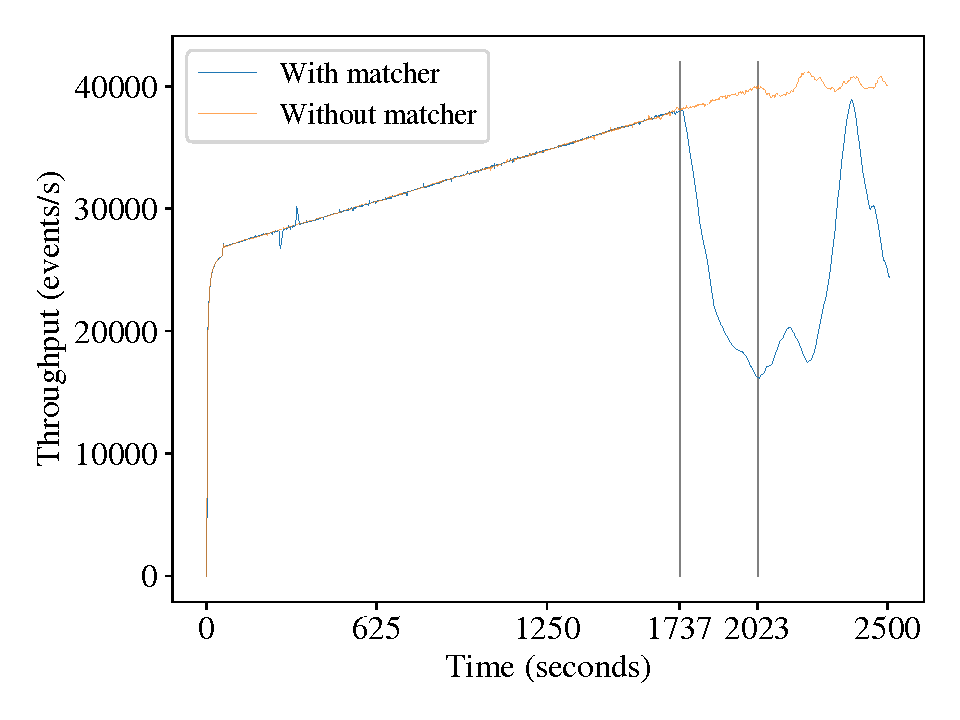
\includegraphics[width=1.0\textwidth]{figures/diffstream/throughput-accelerated.pdf}
        \caption{}\label{diffstream:fig:throughput}
    \end{subfigure}%
    \begin{subfigure}[t]{0.33\textwidth}
        \centering
        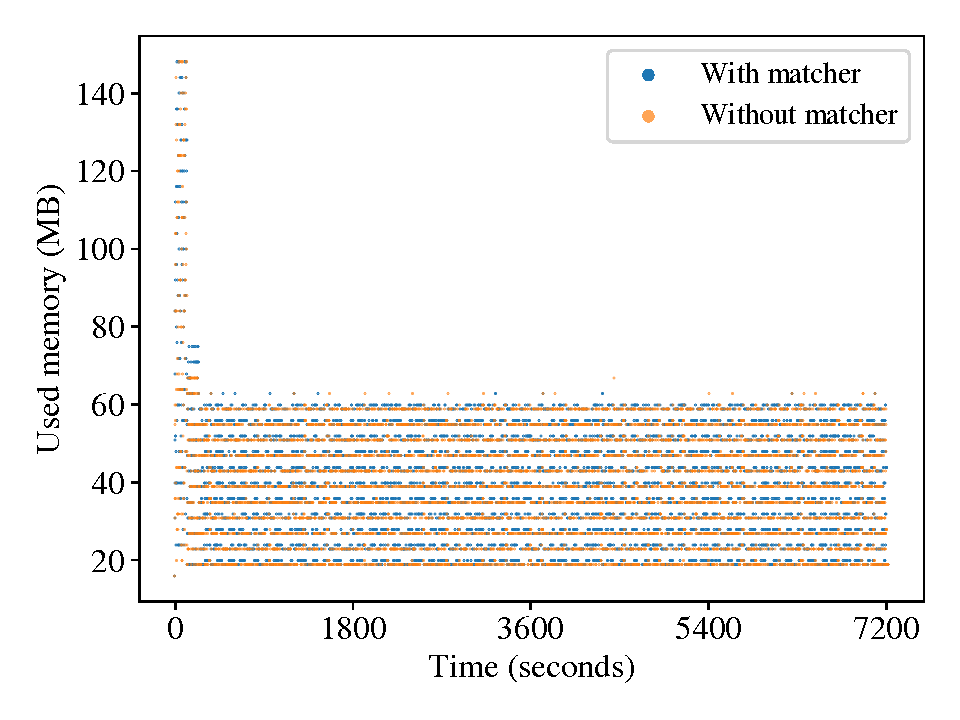
\includegraphics[width=1.0\textwidth]{figures/diffstream/used_memory_in_time.pdf}
        \caption{}\label{diffstream:fig:memory-in-time}
    \end{subfigure}%
    \begin{subfigure}[t]{0.33\textwidth}
        \centering
        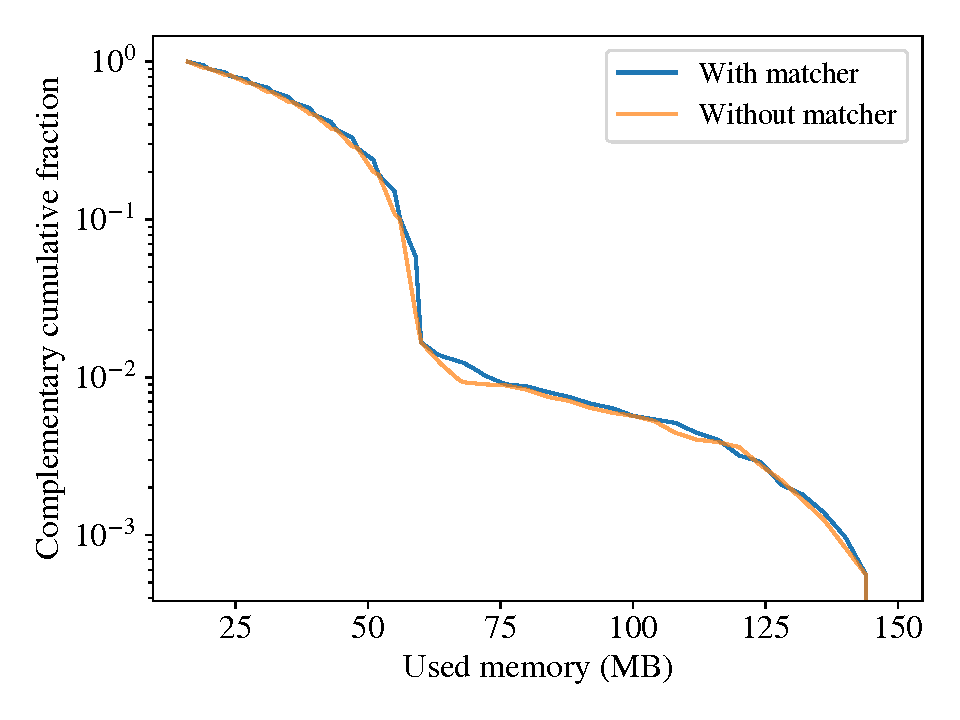
\includegraphics[width=1.0\textwidth]{figures/diffstream/memory_ccdf.pdf}
        \caption{}\label{diffstream:fig:memory-ccdf}
    \end{subfigure}%
    \\
    \begin{subfigure}[t]{0.33\textwidth}
        \centering
        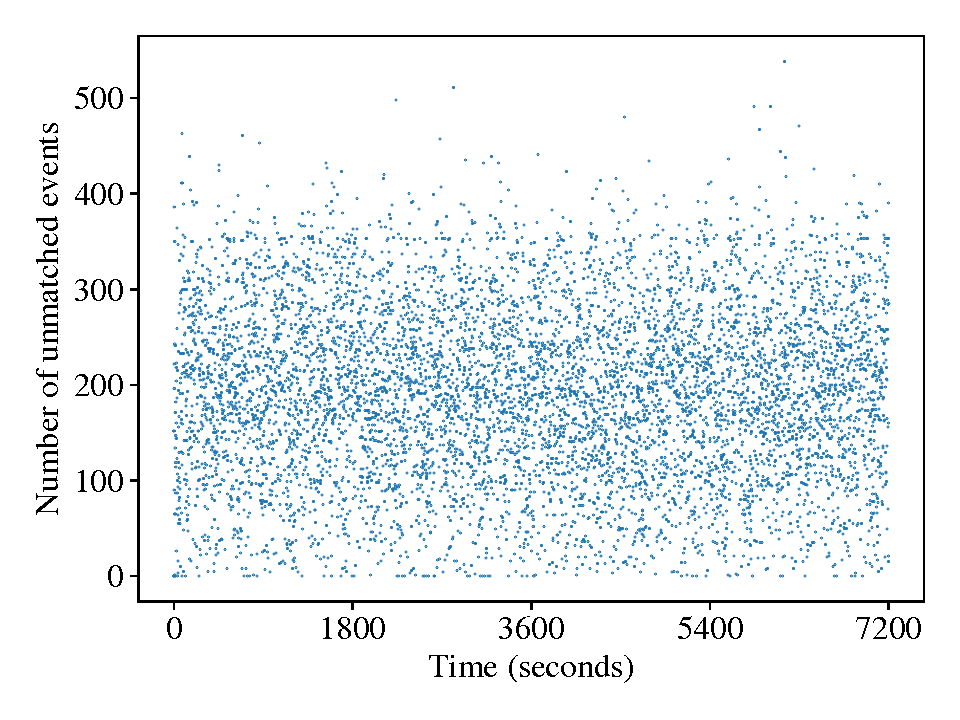
\includegraphics[width=1.0\textwidth]{figures/diffstream/unmatched_in_time.pdf}
        \caption{}\label{diffstream:fig:unmatched-in-time}
    \end{subfigure}%
    \begin{subfigure}[t]{0.33\textwidth}
        \centering
        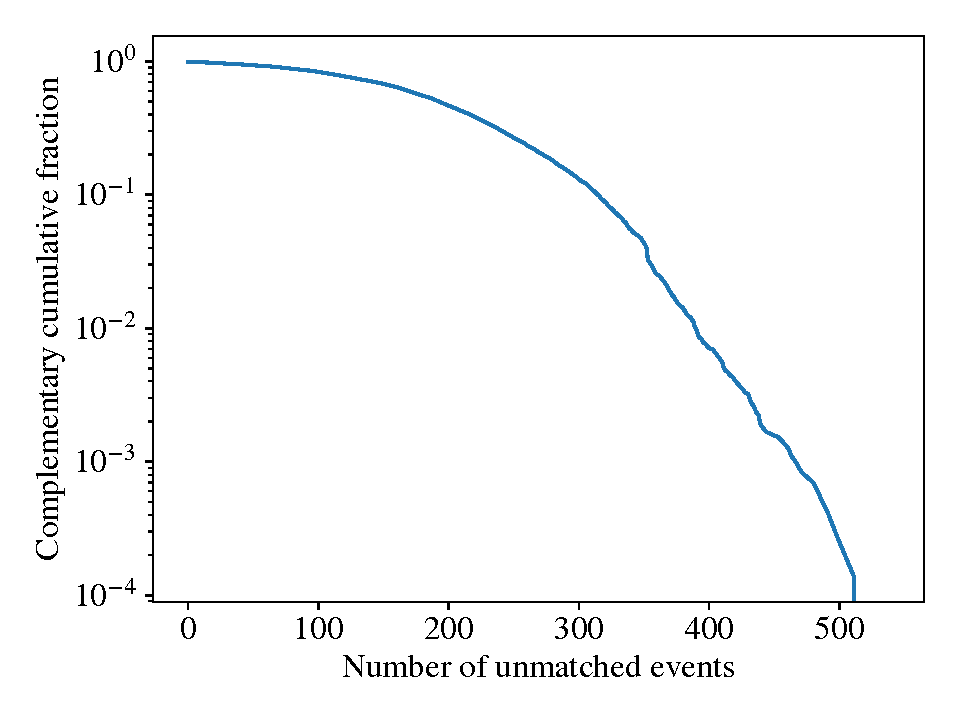
\includegraphics[width=1.0\textwidth]{figures/diffstream/unmatched_ccdf.pdf}
        \caption{}\label{diffstream:fig:unmatched-ccdf}
    \end{subfigure}%
    \begin{subfigure}[t]{0.33\textwidth}
        \centering
        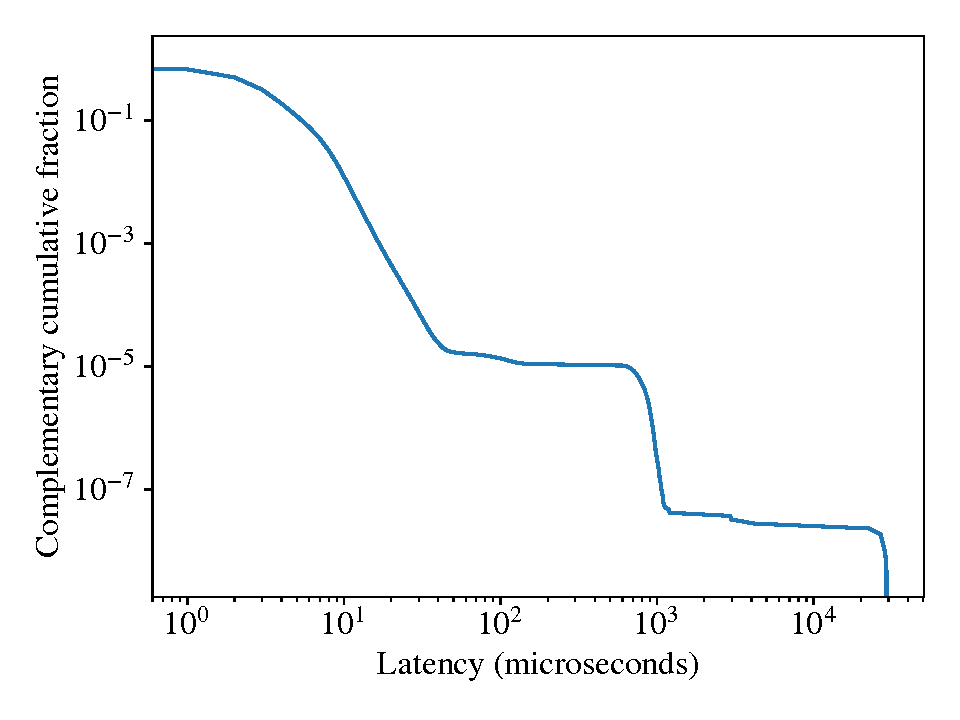
\includegraphics[width=1.0\textwidth]{figures/diffstream/latencies.pdf}
        \caption{}\label{diffstream:fig:latencies}
    \end{subfigure}
    \caption[Performance case study results (Yahoo streaming benchmark).]{Results of the fourth case study: performance measurements of monitoring an application with DiffStream on the Yahoo streaming benchmark over a span of 2 hours, compared to the same application without the DiffStream matcher.}
\label{diffstream:fig:online-perf-results}
\end{figure}

To answer Q1, we modified the ad event producer to steadily increase
the input rate over time. We then executed two experiments: one with the
matcher and one without it. (We simulated the absence of the
matcher with a dummy matcher that ignores every event.) Both
experiments started with an input rate of 40,000 events/s and
the acceleration of 10 events/s$^2$ and ran for 2,500 seconds, allowing the
input rate to increase to 65,000 events/s. The expected ideal throughput of
the matcher is $2/3$ of the input rate due to (i) the duplication
for the two versions of the program, and (ii) the filtering step, which filters
approximately $2/3$ of the events and leaves $1/3$ that finally reach
the matcher. The measured throughput is shown in \Cref{diffstream:fig:throughput}.
Initially, in both experiments the measured throughput matches the ideal
throughput. After 1,737 seconds, the experiment with the matcher reaches
the throughput of 38,072 events/s, after which it rapidly drops and starts
fluctuating. In the experiment without the matcher, the throughput continues
to rise with the input rate until it reaches 40,082 events/s after 2,023 seconds,
after which it also starts fluctuating. Thus, using the matcher results in
approximately 5\% decrease in the maximal throughput.

To answer Q2 and Q3, we implemented a rudimentary memory profiler
that outputs the total heap memory used by the Java Virtual Machine running
the Flink program in 1-second intervals. In addition, we measured the
latencies of the matcher by measuring the time it takes to process each
event; we stored the latencies in a file during execution. We executed
two experiments, with and without the matcher, with a constant input rate
of 45,000 events/s and the duration of 7,200 seconds (2 hours). The input
rate of 45,000 events/s translated into the throughput of 30,000 events/s,
which was stable during the execution.

\Cref{diffstream:fig:memory-in-time} shows a scatter plot of the memory samples taken
during execution. In particular, the total memory used by the program
stays bounded throughout the duration of the experiment. \Cref{diffstream:fig:memory-ccdf}
visualizes the same information in a different way: for an amount of used
memory $x$ on the $x$-axis, the corresponding value on the $y$-axis is
the fraction of memory samples that exceed $x$. The two figures together
show that there is virtually no difference in the memory usage in the two
experiments.
We get a more fine-grained view if we look at the number of unmatched events
that the matcher stores during execution. \Cref{diffstream:fig:unmatched-in-time} shows
a scatter plot of samples of unmatched events taken in 1-second intervals
during execution. In particular, in almost all samples, the number of unmatched
events is below 500. This is even more clearly illustrated in
\Cref{diffstream:fig:unmatched-ccdf}, which shows the fraction of samples exceeding
the given number of unmatched events. Thus, to answer Q2, the memory
footprint of the matcher is bounded and negligible relative to the memory
used otherwise and the throughput of 30,000 events/s.

Finally, to answer Q3,
\Cref{diffstream:fig:latencies} shows the fraction of recorded latencies
that exceed a given number of microseconds.
The mean latency is 2 microseconds.
While the maximal latency is 30 milliseconds, this is rare:
$98.77\%$ of latencies
are at most 10 microseconds, and $>99.99\%$ of latencies are at most
100 microseconds.

\emph{Summary.} The results show that the overhead of running DiffStream in practice is low.
First, the matcher results in a modest $5\%$ reduction in maximal throughput.
Second, the memory usage is stable over time and reflects the theoretical optimality for applications where drift between the two streams is bounded:
the number of unmatched elements is $<1.67\%$ compared to the number events that it processes.
Finally, the latency of the matcher is at most 100 microseconds in $>99.99\%$ of cases, which competitively meets streaming performance standards.

\section{Discussion}
\label{diffstream:sec:conclusion}

As presented, the input to DiffStream consists of the two programs as well as
a \emph{dependence relation} which is used to describe which output
events must be produced in order, and an optional custom equality
which is used to compare output events.
It is also possible to view DiffStream as being a runtime assertion checker: it checks assertions of the form
\[
\texttt{assert s1 == s2}
\]
where \texttt{s1} and \texttt{s2} are streams of a given stream type $S$, and $==$ is stream equivalence $\equivtype{s_1}{s_2}{S}$. Moreover, it does this as efficiently as possible in a streaming complexity sense.

This is how I like to view the library today; an online stream diff calculator. Given a generator and two versions of the program under test, asserting stream equality on their outputs is the usual use case for DiffStream. However, there are other use cases for an equality test, such as validating that a result stream computed by two different nodes is the same.

Keeping in mind the stream-diff-calculator view, here are some possibilities for extension that I currently think would be promising:
\begin{itemize}
  \item First, the library could be extended not just to check equality (yes or no answer), but to truly compute a diff between the two streams. The core algorithmic problem would be more challenging.
  \item Second, the algorithm could be revised to avoid the worst-case behavior described in \Cref{diffstream:sec:practical-bounds} if we relax a simple requirement: if we require that differences between the two streams are detected \emph{with high probability}, rather than necessarily. In particular, one could make use of hash functions for this purpose. Consider the failure case where the two input streams are bags. Rather than store the full diff of the input streams, could one just store a sum of the hash values of each bag? It is mathematically rare for $\sum_{s \in S_1} \texttt{hash}(s) = \sum_{s \in S_2} \texttt{hash}(s)$ unless $S_1 = S_2$.
\end{itemize}

An honest limitation of DiffStream is that it focuses on bugs due to parallelism. In fact, this is only a small class of all bugs; and even smaller if we exclude bugs that could be caught through unit testing without requiring nontrivial dependence relations. In future work, it would be prudent to target other classes of bugs, including those due to node or network faults.
Additionally, we would like to generalize the definition of correct behavior, which currently assumes that the output should be determined up to allowed reordering and equality of data items. There are cases where this is too strong, for instance when operations are approximate or randomized.

Another limitation of DiffStream is that it does not address the problem of input data generation, but instead uses an off-the-shelf generator (JUnit-QuickCheck).
There is an interesting problem of generating input streams of a type $S$,
taking into account the type of $S$, which we don't really consider in this work.
To clarify, DiffStream does check for type safety and determinism, but only on a specific example trace at a time. That is, on an input stream and an equivalent input stream, it can check whether the outputs are equivalent.
But, as with all runtime testing techniques, this only allows testing finitely many input traces.
This is the reason for the \Partial{} entries in \Cref{fig:operator-properties-chapter-table}.

DiffStream is open source and is available \githubref{https://github.com/fniksic/diffstream}{on GitHub}.
